%%%%%%%%%%%%%%%%%%%%%%%%%%%%%%%%%%%%%%%%%%%%%%%%%%%%%%%%

%%%  Welcome to the Cell Press LaTeX template,
%%%  version 1.10. This is a minimalist template
%%%  to help you organize your article for
%%%  publication at Cell Press. PLEASE NOTE:

%%%  (1) If you submit your final manuscript materials
%%%  in LaTeX format, our typesetters will prepare
%%%  a Word file for use in production. This conversion
%%%  process allows us to copyedit your paper, fix
%%%  any typos, and add formatting and tagging. The
%%%  conversion process will add approximately 3
%%%  business days to the production timeline.
%%%  Authors using LaTeX should keep this in mind
%%%  when considering deadlines.

%%%  (2) Keep your LaTeX files as simple as possible.
%%%  Avoid the use of elaborate local macros and/or
%%%  customized external style files. If you need
%%%  additional macros, please keep them simple and
%%%  include them in the actual .tex document preamble.
%%%  Source code should be set up so that all .sty
%%%  and .bst files called by the main .tex file are
%%%  in the same directory as the main .tex file.

%%%  (3) Cell Press publishes more than 40 journals,
%%%  some of which may have different or additional
%%%  formatting requirements not specified in this
%%%  template. When revising your paper before
%%%  acceptance, please review the formatting
%%%  guidelines, including the Final Files Requirements,
%%%  for the journal you are publishing with.

%%%  Please send feedback on this template to lshipp@cell.com.

%%%%%%%%%%%%%%%%%%%%%%%%%%%%%%%%%%%%%%%%%%%%%%%%%%%%%%%%

\documentclass[12pt,letterpaper]{article}
\usepackage[a4paper, total={7in, 10in}]{geometry}
\renewcommand{\familydefault}{\sfdefault}
\usepackage{graphicx}
\usepackage{helvet}
\usepackage{authblk}
\usepackage{hyperref}
\usepackage{booktabs}
\usepackage{amsmath}
\usepackage{amssymb}
\usepackage{orcidlink}
\usepackage[super,comma,sort&compress]
   {natbib}\bibliographystyle{numbered}
\usepackage[right]{lineno} \linenumbers

\graphicspath{ {../figures/} }

\makeatletter
\renewcommand{\maketitle}{\bgroup\setlength{\parindent}{0pt}
\begin{flushleft}
  \textbf{\@title}

  \@author
\end{flushleft}\egroup}
\makeatother

%%%  Insert title below; leave date empty.

\title{Inferring the Recombinant Genealogy of a Pandemic Pathogen in Real Time}
\date{}

%%%  Author first and last names should be spelled
%%%  out in their entirety (do not abbreviate "J.H.
%%%  Watson" unless this is how the author's name
%%%  always appears). Middle initials are OK. Do
%%%  not include titles, positions, or degrees.

%%%  Use numbered footnotes to indicate institutional
%%%  affiliations. Authors may have multiple
%%%  institutional affiliations, and affiliations
%%%  may be shared among multiple authors.

%%%  After the institutional affiliations, numbered
%%%  footnotes may be used to indicate an author's
%%%  present address, equal contribution status,
%%%  and/or senior author status.

%%%  The final numbered footnote should indicate
%%%  which author is the lead contact (required).
%%%  One author must be designated as the lead contact.
%%%  There can be no more than one lead contact.

%%%  Corresponding authors should be indicated with
%%%  asterisks (*). Use 2 asterisks (**) for the
%%%  second-listed corresponding author, 3 (***) for
%%%  the third-listed, and so on. The lead contact
%%%  must be a corresponding author. Additional
%%%  authors may also serve as corresponding authors.

\author[1,\orcidlink{0000-0000-0000-0000}]{First Last}
\author[1,2]{First Middle Last}
\author[2,3]{First M.M. Last}
\author[3,*]{First Last, Jr.}
\author[3,4,5,**]{F. Middle Last}


%%%  Institutional affiliations should contain the
%%%  following information at minimum: department(s)/
%%%  subunit(s), institution, city, state/region (if
%%%  applicable), and country.

\affil[1]{University A, London SW7 2AZ, UK}
\affil[2]{Department B, University B, Toronto, ON M5S 3H6, Canada}
\affil[3]{Division C, Department C, University C, Cambridge, MA, USA}

\affil[4]{Senior author}
\affil[5]{Lead contact}

%%%  List only one email address per corresponding author.

\affil[*]{Correspondence: first.last.jr@university.edu}
\affil[**]{Correspondence: f.middle.last@university.edu}


\begin{document}

\maketitle

\section*{SUMMARY}

%%% The summary (abstract) should consist of a single paragraph of 150 words or fewer.
%%% This is the SMBE abstract. We can rewrite or work off of it, but it needs to be shorter.
Widely used phylogenetic methods to study SARS-CoV-2 evolution assume that genetic recombination is negligible and
viral relationships can be represented by a single tree.
However, important SARS-CoV-2 recombinant lineages have emerged.
A more suitable approach is to use ancestral recombination graphs (ARG),
which jointly model recombination, mutation, and genetic inheritance in a cohesive framework.
Recent computational advances have made ARG inference possible for datasets of millions of genome sequences.
Building on these new advances, we have developed sc2ts, a scalable method to simultaneously detect recombinants and
reconstruct ARGs from heterochronous SARS-CoV-2 genome sequences.
Using sc2ts, we inferred an ARG of 2.48 million genomes sampled from January, 2020 to February, 2023.
We find that this pandemic-scale ARG unifies known features of SARS-CoV-2 evolution —
the backbone phylogeny, mutational spectra, and major recognized recombinants.
This ARG enables us to explore the evolutionary origins of known and novel recombinants.
Furthermore, the ARG is compactly stored in the tree sequence format using the tskit library and
can be analyzed efficiently and interactively using standard Python tools on a typical laptop.
This combination of capabilities makes sc2ts a powerful tool
for studying the recombination and mutation processes driving SARS-CoV-2 evolution.


\section*{KEYWORDS}

%%%  Include up to 10 keywords, separated by commas.
%%%  Keywords entered in EM are not carried over; only
%%%  keywords included in the main text will be used
%%%  in the final article metadata. Please note that
%%%  for some journals, keywords are chosen by the editors.

ancestral recombination graphs, population genetics, recombination, tree sequence, SARS-CoV-2


\section*{INTRODUCTION}

%%% No subheadings, please. Use of abbreviations should be kept to a minimum,
%%% and nonstandard abbreviations should be defined when first used in the text.

The genomic revolution has brought about a paradigm shift
in the way we study the evolution and spread of pathogens,
allowing real-time tracking of pathogens over time and space.
During the COVID-19 pandemic, thousands of SARS-CoV-2 genome sequences were generated daily,
quickly overwhelming typical phylogenetic approaches.
Although real-time phylogenetic methods now exist to cope with this flood of genomic data
(e.g., UShER\cite{Turakhia2021,DeMaio2023}),
we lack methods to build phylogenies that can integrate recombination
in the face of ongoing sampling of infected cases.

UShER is a maximum parsimony method developed during the pandemic to infer phylogenies
from large numbers of densely sampled SARS-CoV-2 genome sequences \cite{Turakhia2021}.
UShER has generated phylogenies updated daily \cite{McBroome2021} and
has proven to be a powerful resource that successfully enabled the world
to keep up with an evolving disease (e.g., through the Nextstrain web portal \cite{Hadfield2018}).
These phylogenies are used to identify and monitor
potentially epidemiologically important “Pango” lineages \cite{Rambaut2020,McBroome2024},
which might have acquired features to become Variants of Concern (VOC),
for example, increased transmissibility, disease severity, and immune escape.
Beyond supporting real-time genomic epidemiology,
UShER phylogenies have been used in a multitude of evolutionary and epidemiological studies of SARS-CoV-2
(e.g., \cite{Karthikeyan2022,Obermeyer2022,Turakhia2022,Bloom2023}).
UShER uses a tree to represent evolutionary change via mutation, assuming no recombination \cite{Turakhia2021}.
However, given extensive evidence for recombination in SARS-CoV-2 \cite{Jackson2021,VanInsberghe2021,Focosi2022,Gutierrez2022,Ignatieva2022,Tamura2022},
the tree-like representation of UShER is no longer tenable.

Ancestral Recombination Graphs (ARGs) are reticulate genealogies that incorporate both mutation and recombination events \cite{Wong2024},
potentially allowing more comprehensive evolutionary representations of SARS-CoV-2 and other viruses undergoing recombination.
Until recently, ARGs lacked software support and sufficiently scalable inference methods to be of practical use.
Recent advances enable ARG inference for tens to hundreds of thousands of human genomes \cite{Kelleher2019,Speidel2019,Zhang2023},
with high levels of recombination.
These advances now enable evolutionary genealogies to be built quickly and at scale, and
there is a surge of excitement in the inference and applications of ARGs \cite{Brandt2024,Lewanski2024,Wong2024,Nielsen2025}.

Previous ARG methods are retrospective \cite{Rasmussen2014,Kelleher2019,Speidel2019,Ignatieva2022,Zhang2023},
reconstructing the past from a sample of genome sequences drawn at one moment in time,
but scientists are increasingly tracking evolutionary change as it happens, accumulating data forward in time.
For example, sequences from daily samples of SARS-CoV-2 were made globally available on a daily basis,
leading to over 17 million sequences in the GISAID database \cite{Shu2017}.

Here, we present
(1) sc2ts, a new method to infer ARGs in real time by building genealogies forward in time, and
(2) an ARG for SARS-CoV-2 with ~2.48 million genome sequences.
We used the “Viridian” dataset, which is purged of various systematic errors and artifacts \cite{Hunt2024} and
show that this ARG is highly congruent to an UShER phylogeny built from the same dataset.
Compared to previously identified recombinants,
we show that this ARG contains the vast majority of epidemiologically relevant signals of recombination,
while adding significant nuance and texture.
This ARG – which captures the major signals of evolution
through phylogenetic relationships, point mutations, deletions, and recombination –
is a resource of unprecedented detail and precision, and
should provide a strong basis for future studies of SARS-CoV-2.


\section*{RESULTS}

%%% The results may be divided with subheadings.
%%% In our view, good subheadings convey information about the findings,
%%% so we encourage you to be specific. For example, "Factor X requires factor Y to function in process Z"
%%% is better than "Analysis of factors X and Y by approach Q."
%%% We recommend that you use similar language in your figure titles for clarity and structural harmony.
%%% Please do not use numbered subheadings. For some formats, ``results and discussion" may be combined under a single heading.

%%% For initial submissions, figures and their titles and legends can be run-in with the text.
%%% For final submissions, the image files must be uploaded as separate files, one complete file per figure. The figure titles and legends should be placed toward the end of the main text, after the declaration of interests. Our typesetters will place the figures and their titles and legends appropriately based on your in-text citations.

%%% To cite/link to display items (figures and tables) and/or sections of the manuscript,
%%% simply write, for example, ``(Figure 1)" or ``see discussion."
%%% Our team will do the rest. Please note that we do not number sections or subsections.

\subsection*{Brief description of sc2ts}

Sc2ts reconstructs an ARG by incrementally adding batches of sequences as they become available
(\ref{fig:methodology}; for details, see STAR Methods).
First, sc2ts infers likely ``copying paths'' connecting each sample in the batch to node(s) in the current ARG
(allowing recombination) using the Li and Stephens (LS) model \cite{Li2003},
which is a Hidden Markov Model (HMM) widely used in human genomics
to approximate the effects of mutation and recombination on genetic inheritance.
As recombination is relatively rare in viruses,
we would expect most samples to copy from a single parent in the ARG.
Recombinant samples, however, copy from two or more parents, with switching (recombination) in the copying path
between the parents resulting in different genomic segments inherited from the different parents.
Next, for clusters within the batch that are inferred to copy from the same ARG node,
sc2ts uses standard phylogenetic techniques to resolve relationships within the cluster.
Finally, sc2ts attaches the phylogenies of the clusters to the current ARG, and
applies parsimony-improving heuristics to address issues introduced by the inherent greediness of this strategy.

Sc2ts uses collection dates to build a time-resolved ARG.
When examining preliminary ARGs, we found samples that introduced large numbers of mutations (and reversions),
likely due to errors in their collection dates
(for example, a large batch of samples dated 31 December, 2020 contains samples from Omicron BA.1,
which is estimated to have emerged in November, 2021; REF).
To preclude adding such “time traveling” samples, we filtered samples by “HMM cost”.
We define the “HMM cost” of a sample to be
the total penalty cost for switches and mismatches (mutations) in its copying path.
We parameterize the LS model such that each mismatch has a penalty cost of one
and a switch has a penalty cost of $k$ (here, set to 4),
which determines how much mutation is favored over recombination when accounting for a sample (\ref{fig:methodology}).
If the HMM cost of a sample exceeds a threshold (here, set to 7),
sc2ts does not immediately add the sample to the ARG.

This approach resulted in preliminary ARGs that had noticeably fewer time travelers,
but we found that it also excluded the major “saltation” events that characterize many VOCs.
These saltation lineages are characterized by a high number of accumulated mutations,
and are hypothesized to emerge from chronic infections
during which the virus is exposed to individual-specific immune selective pressures \cite{Markov2023}.
Though uncommon, such lineages drove large epidemic waves during the pandemic (notably Alpha, Delta, and Omicron).
To distinguish time travelers with erroneous dates from true saltation lineages,
we reevaluate the evidence for each lineage with a high HMM cost as additional samples are added.
If on subsequent days these lineages form a sufficiently large group of samples,
sc2ts adds the group back to the ARG.
This “retrospective sample grouping” successfully captured the emergence of most saltation lineages (Figure SX).
The emergence of the Delta, BA.1, and BA.2 lineages required some manual intervention,
in which specific "seed" samples were identified for unconditional inclusion
(for details of how seed samples were chosen, see STAR Methods).
First arising in geographic regions with low sampling density,
the initial origins of these VOC are challenging to infer (REF).

\begin{figure}[h]
    \centering
    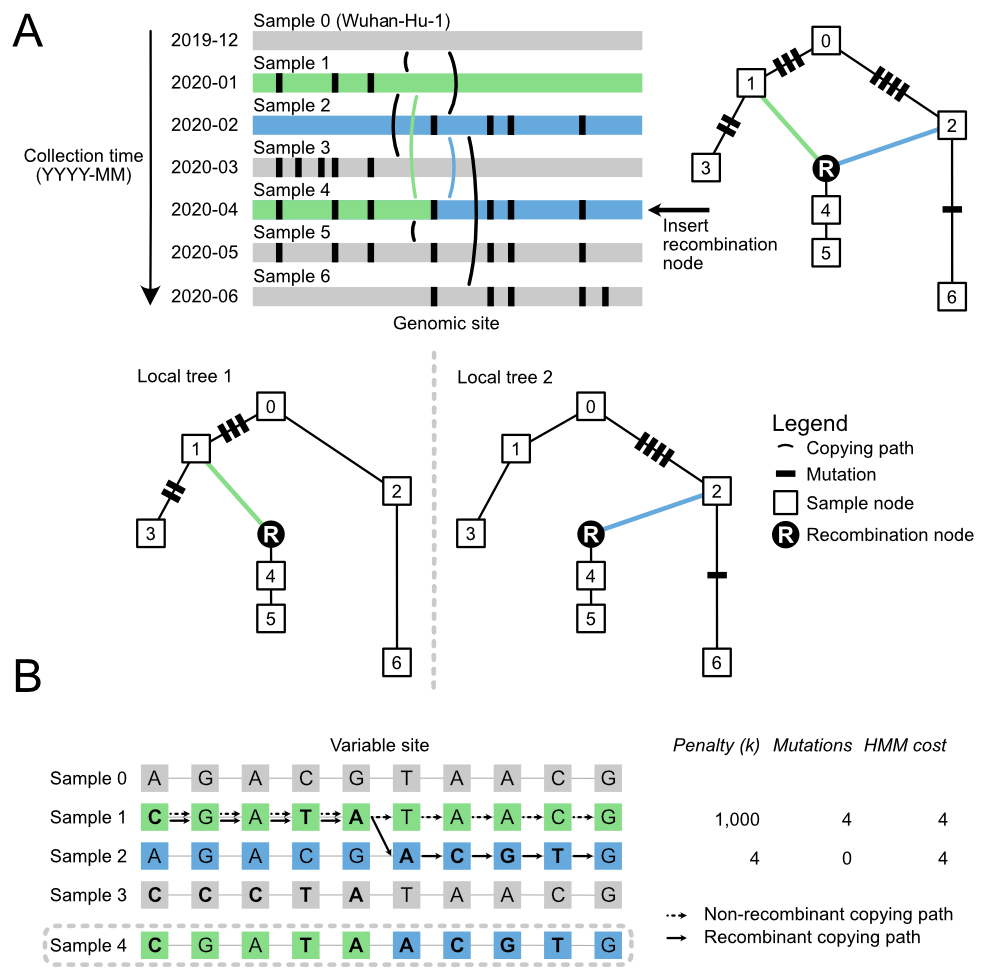
\includegraphics[width=0.85\linewidth]{methodology.png}
    \caption{Schematic overview of sc2ts. (A) Procedure to build an ARG by incrementally updating it with samples sorted by collection dates. Sample 0 is used to initialize the ARG as the root. Next, Sample 1 is attached, mapping mutations onto the new branch to explain it. When Sample 4 is detected as a recombinant, a node representing the recombination event is inserted with two edges connecting to its parents, with Sample 4 itself attached to this node as its child. The resulting ARG contains two local trees, one on each side of the inferred breakpoint. (B) Copying paths for Sample 4 inferred under the LS model while allowing recombination ($k = 4$) or disallowing it ($k = 1000$).}
    \label{fig:methodology}
\end{figure}


\subsection*{A comprehensive representation of SARS-CoV-2 evolution}

Using sc2ts, we built an ARG of ~2.48 million-samples spanning the COVID-19 pandemic.
Inference took 21 days on a server equipped with dual EPYC (details) and 500 GB of RAM (~5 CPU years; Figure SX).
The ARG contains 2,689,054 nodes representing the genealogical relationships
among 2,482,157 sampled genomes in the Viridian v04 dataset,
which were collected from January 01, 2020 to February 20, 2023 \cite{Hunt2024}.
Of the nodes, 855 represent recombination events,
of which 356 have a minimum of four loci supporting the non-focal parent on both sides of the breakpoint
(we refer to these as “robust” recombination events, Figure SX; see Document S1),
reflecting the overwhelming tree-like structure of SARS-CoV-2 evolutionary history.

The ARG represents the full evolutionary history of SARS-CoV-2 and
is in close agreement with the state-of-the-art UShER phylogeny built using the Viridian dataset \cite{Hunt2024}.
First, we validated the broad structure of the ARG against the UShER phylogeny \cite{Hunt2024}
by pruning both down to representative samples for 1097 deeply-sampled lineages (STAR Methods).
Tanglegrams reveal that the ARG captures known phylogenetic relationships
both within sublineages and at the level of major lineages (including VOCs),
with good agreement between the phylogenetic bipartitions in the ARG and the UShER phylogeny (Figure S2).
Next, we compared the high-level properties of the sc2ts and UShER inferences from the Viridian dataset
by pruning both to their intersection of 2,475,418 samples and 27,431 sites.
Remarkably, given the differences in inference methods and data processing pipelines,
they are almost identically parsimonious,
with sc2ts requiring 4,208 (0.23\%) fewer mutations than UShER (1,843,132 for UShER vs 1,838,924 for sc2ts).
We also compared the mutational spectra of major VOCs in the ARG
against the mutational spectra computed from the UShER phylogeny (STAR Methods),
finding a close match to previous reports \cite{Bloom2023} (Figure S3).

Input genome alignments are masked in sc2ts
so that deletions and ambiguous bases are treated as missing data by the HMM,
and once the samples are incorporated into the ARG,
these bases are imputed to carry the values inherited by the node in question.
Deletions are an important part of SARS-CoV-2 evolution \cite{Jeronimo2023}, however,
and to incorporate them into the ARG we identified a set of [XXX] sites
most frequently involved in deletions [cite source?]
and post-hoc mapped alignment data for these sites to the ARG using parsimony.
Although sites are treated independently in this approach,
the approximation successfully identified the most frequent deletions,
such as the recurrent 21991-21993 (for more details, see Document S1).
The node representing the origin of Alpha, with 290,407 descendants,
is correctly associated with key lineage-defining deletions:
11288-11296 (ORF1A del3675-3677),
21765-21770 (Spike del69-70),
21991-21993 (Spike del144), and
28271 (non-coding).
The Spike 69-70 deletion, which causes S-Gene Target Failure \cite{Walker2021},
also emerges twice in the origin of Omicron -
in the node leading to the BA.1 variant (342,099 descendants),
and the node leading to the BA.4 variant (189,746 descendants).
To speed up inference and to avoid issues caused by sites enriched for errors [citation?],
sc2ts masks out a set of 100 sites identified as the most highly homoplasic
by running on a subset of the data (STAR Methods).
Of these sites, 9 are in the set of [1XX] “problematic sites” masked by UShER \cite{Hunt2024}.
In addition to remapping the data for sites identified as being involved in deletions,
we added mutations for XX of these highly recurrent sites
that are used in Pango designation \cite{Rambaut2020} by post-hoc parsimony.
Each node in the ARG was then assigned to one of 2026 Pango lineages using pangolin (STAR Methods).
All but 8293 sampled sequences (0.33\%) agreed with the source sequences in terms of Pango lineage assignment
(comparable to the 0.27\% disagreement between pangolin-data versions 1.21 and 1.29 in the source Viridian metadata).
A majority of these lineages (1469 of 2058) have monophyletic origins within the ARG,
increasing to 1779 (86\%) when we allow for multiple sibling origination nodes (Table SX; Document S1).


\subsection*{Epidemiologically relevant recombinant lineages}

As new data became available during the pandemic,
volunteers continually detected recombinants which might have concerning features,
particularly increased transmissibility, disease severity, and
ability to escape natural or vaccine-induced immunity (e.g., \cite{Tamura2022}).
The process of gathering evidence for and characterizing such recombinants is manual,
involving visual inspection of phylogenies for unusual branches
caused by forcibly placing recombinant sequences onto them,
typically followed by visual analysis of genome sequence alignments
to identify parental lineages and breakpoint locations.
This process has resulted in the designation of recombinant Pango lineages
(whose aliases begin with an “X”), to which we refer as “Pango Xs”.
Below, we summarize our analysis of the Pango Xs in the ARG
(for extended analyses, see Document S1 and Document S2).

We find strong evidence for the recombination events leading to 17 Pango Xs in the ARG (Table 1),
which passed the detection-level sc2ts quality control filters (Figure S1).
These events are supported by
high numbers of averted mutations (Table 1) and
high numbers of loci matching their suggested parents (see their copying patterns in Figure SX).
Among these Pango Xs are
XA, which is the first designated Pango X that showed signs of community transmission \cite{Jackson2021}, and
XBB, which escaped vaccine-induced immunity and gained global prevalence \cite{Tamura2022}.
The recombinant origin of XA is well explained in the ARG by two parents and one mutation (\ref{fig:subgraphs}; Table 1),
with sc2ts correctly identifying its parental Pango lineages and breakpoint location.

Furthermore, some of the Pango Xs above originate from shared recombination events in the ARG (Table 1).
An example of a set of “nested” closely related Pango Xs consists of XZ, XAC, XAD, XAE, and XAP,
which descend from a single recombination event rather than five independent events in the ARG (\ref{fig:subgraphs}).
These Pango Xs were designated around the same time.
These results highlight that the ARG can help clarify the relationships between recombinants,
allowing more precise interpretation of evidence for recombination.

Sc2ts identified 12 Pango Xs in the ARG as non-recombinants (Table 1),
on the basis of the HMM and available data.
For all these Pango Xs, the number of recombination-informative sites
fell below our threshold of detection (i.e. $k = 4$ in the HMM).
The fact that most of these Pango Xs (except XAJ and XAN) differ from a single parent node in the ARG
by at most three mutations (Table 1) strongly supports their origins as non-recombinants.
For example, the closely related XN and XAU can be explained
by two mutations and one mutation in the ARG, respectively (\ref{fig:subgraphs}).
%%% TODO: Say something about XAJ and XAN.
However, sc2ts did not detect several Pango Xs (XB, XP, and XAJ) as recombinants
because the HMM treated characteristic deletions as missing data.

\begin{figure}[h]
    \centering
    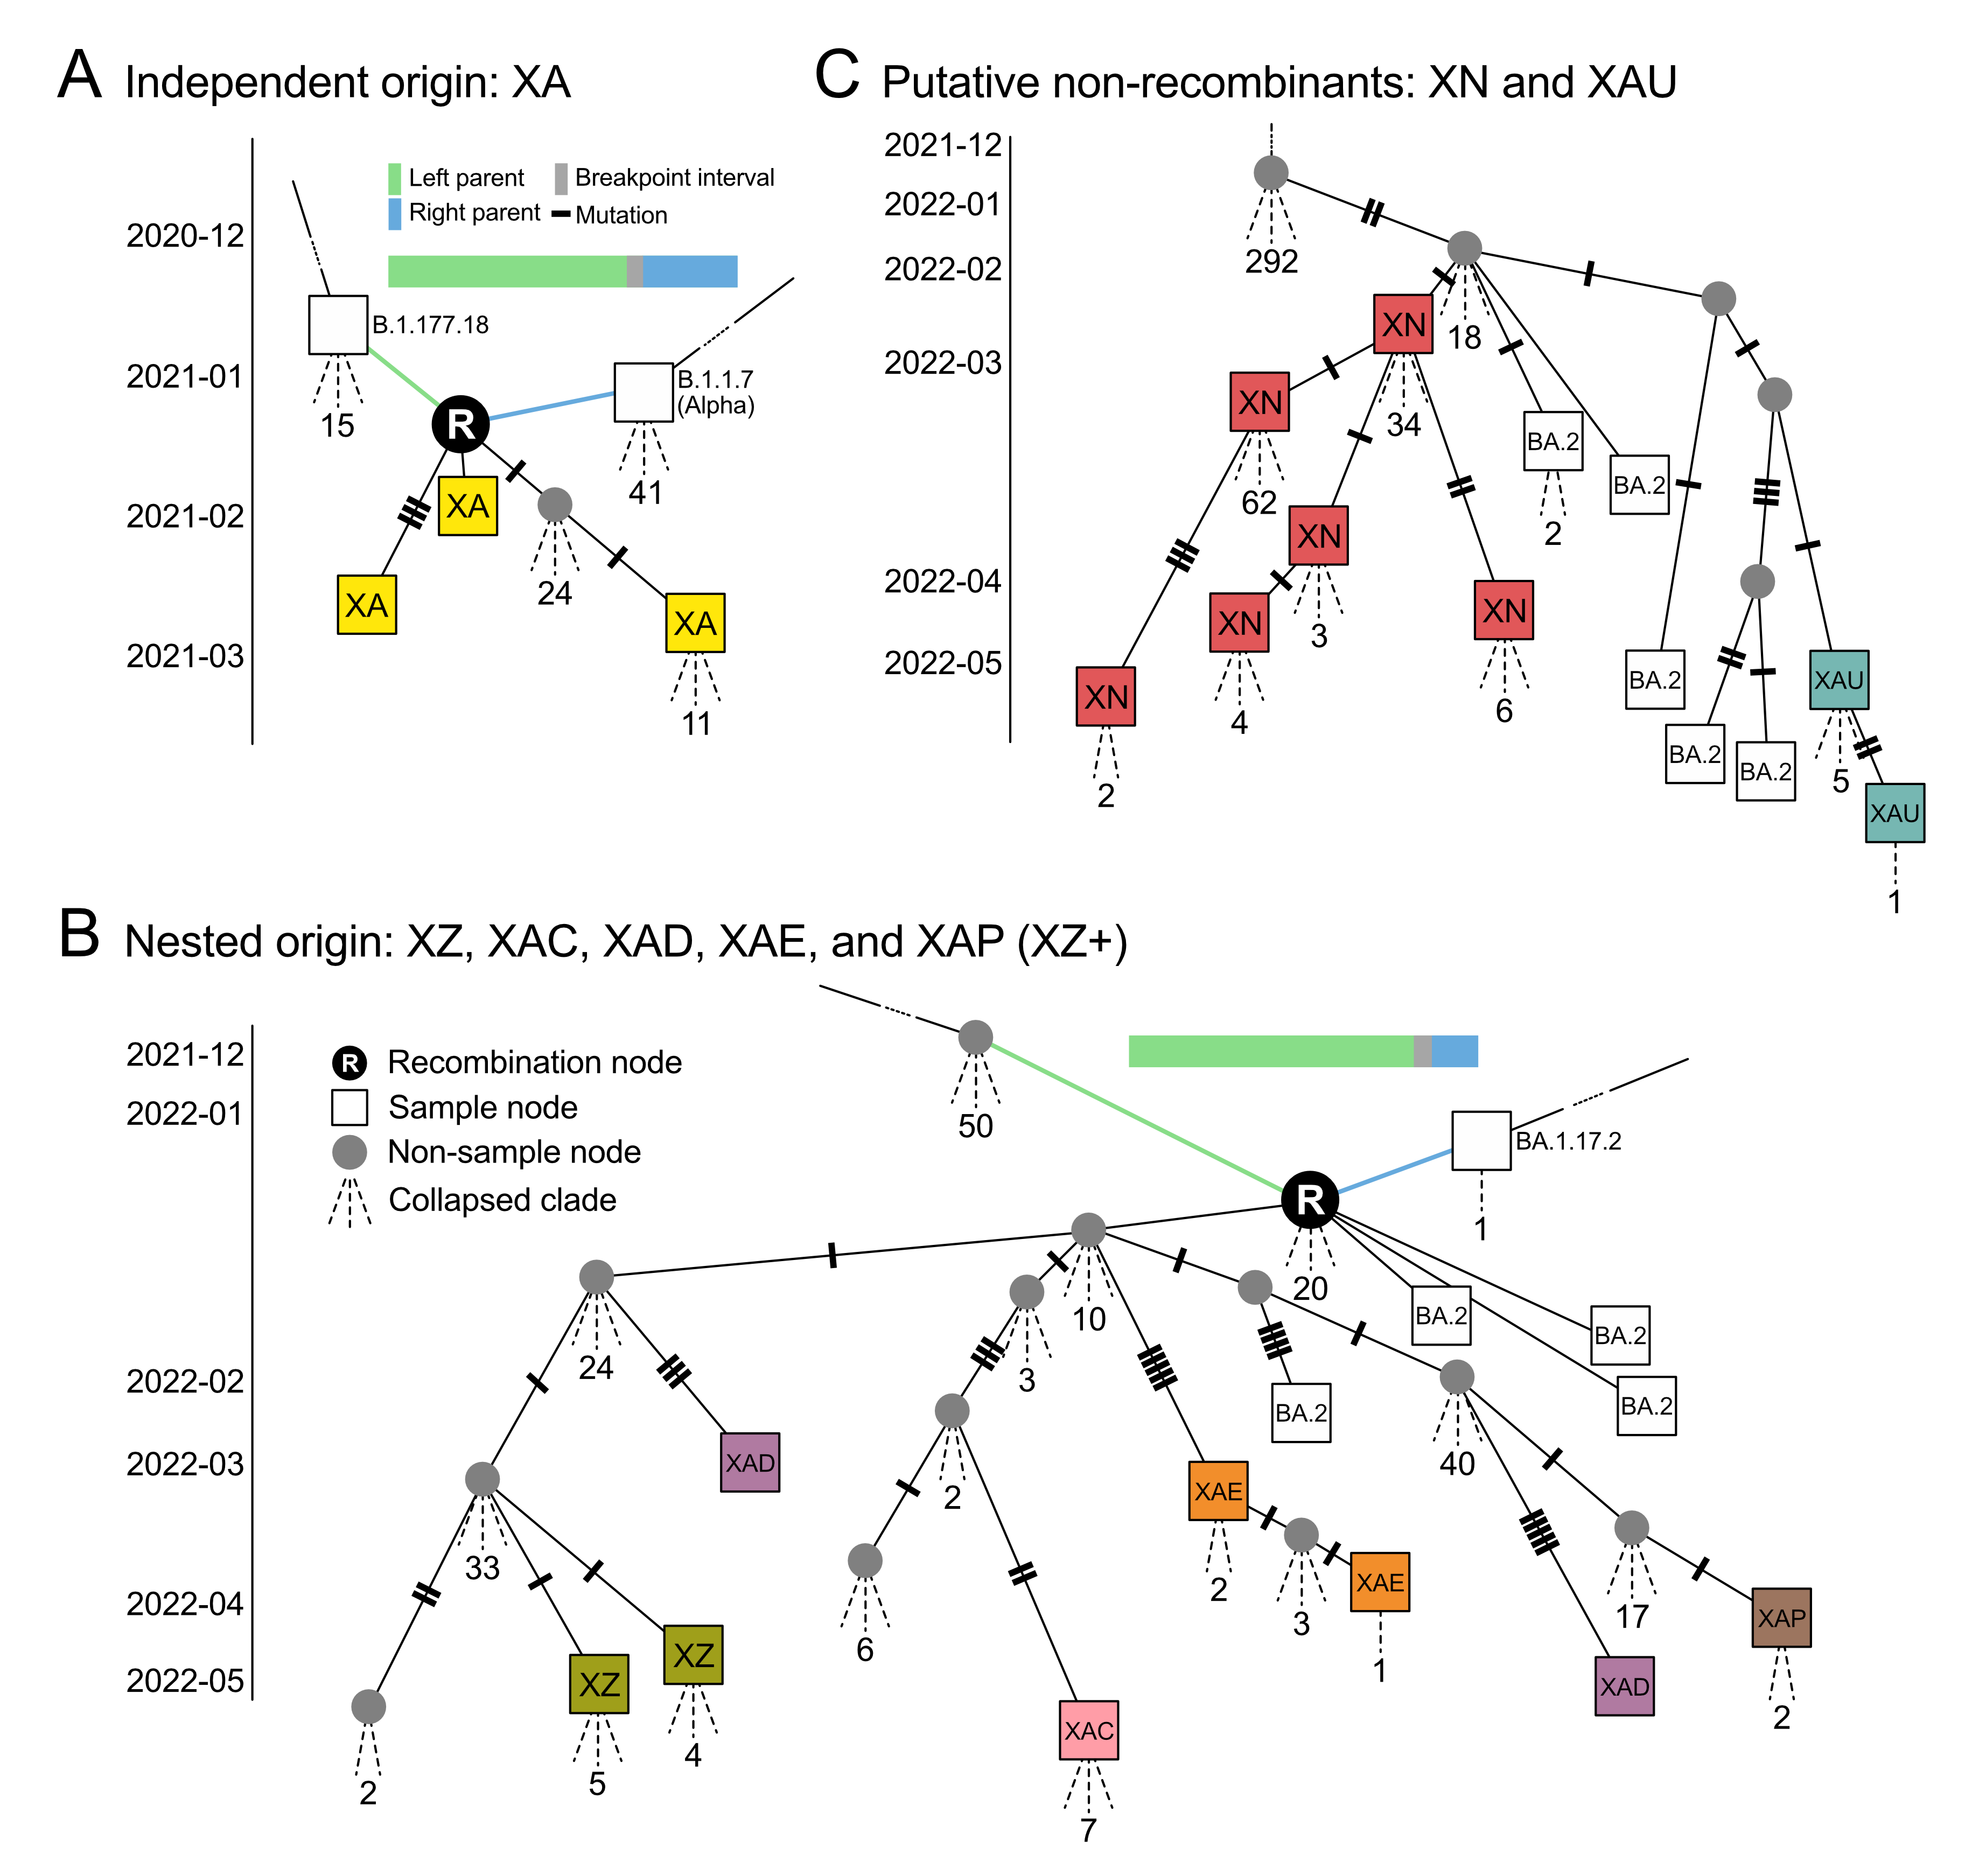
\includegraphics[width=0.85\linewidth]{pango_x_subgraphs.png}
    \caption{Illustrative subgraphs in the ARG. Subgraphs around the XA-associated recombination node (depicted as an encircled R) (A); the recombination node associated with a group of “nested” Pango Xs (B); and the MRCA of the putative non-recombinants XN and XAU (C). For more detailed visualizations of these subgraphs, see Document S2.}
    \label{fig:subgraphs}
\end{figure}

\subsection*{Table 1. Recombination events associated with Pango Xs.}


% This table is generated by the notebook tab_pango_x_events
\begin{table}
\caption{ARG events associated with Pango X lineages.
Each row corresponds to the oldest node assigned the specified
Pango lineage and the ancestor of all nodes assigned that label
(except XBB, XBB.1 and XM; see STAR methods). [MORE DETAILS]
\label{tab:pango_x_lineages}}
\begin{tabular}{lrlrrrrr}
\toprule
pango & samples & extra & muts & root & recomb & t recomb & p recomb \\
\midrule
XA & 39 & \{\} & 1 & 122444 & 122444 & 0 & 0 \\
XBB & 6452 & \{BA.2:1\} & 14 & 1396207 & 1396207 & 0 & 0 \\
XBB.1 & 2 & \{\} & 1 & 1429711 & 1429711 & 0 & 0 \\
XBD & 30 & \{\} & 0 & 1378208 & 1378208 & 0 & 0 \\
XBF & 185 & \{\} & 3 & 1420385 & 1420385 & 0 & 0 \\
XBG & 25 & \{\} & 2 & 1291970 & 1291970 & 0 & 0 \\
XBR & 1 & \{\} & 2 & 1420166 & 1420166 & 0 & 0 \\
XC & 5 & \{\} & 1 & 414488 & 414488 & 0 & 0 \\
XF & 16 & \{\} & 1 & 946761 & 946761 & 0 & 0 \\
XG & 3 & \{\} & 3 & 1083412 & 1083412 & 0 & 0 \\
XL & 64 & \{\} & 1 & 1034619 & 1034619 & 0 & 0 \\
XM & 26 & \{BA.2:16, XAL:3\} & 0 & 1003220 & 1003220 & 0 & 0 \\
XQ & 55 & \{BA.2:37, $\star$\} & 3 & 1058654 & 1058654 & 0 & 0 \\
XS & 17 & \{\} & 1 & 1000242 & 1000242 & 0 & 0 \\
XW & 32 & \{\} & 1 & 1159411 & 1159411 & 0 & 0 \\
XY & 23 & \{\} & 2 & 1187989 & 1187989 & 0 & 0 \\
\midrule
XAA & 17 & \{\} & 3 & 1183815 & 1058654 & 33 & 6 \\
XAE & 9 & \{\} & 7 & 1118099 & 964555 & 47 & 2 \\
XAF & 1 & \{\} & 8 & 1314603 & 1177107 & 140 & 5 \\
XAG & 6 & \{\} & 4 & 1248341 & 1058654 & 55 & 6 \\
XAL & 3 & \{\} & 2 & 1264107 & 1003220 & 66 & 3 \\
XAM & 21 & \{\} & 3 & 1240312 & 1058654 & 43 & 6 \\
XAN & 7 & \{\} & 5 & 1301399 & 1189192 & 114 & 4 \\
XAP & 20 & \{\} & 1 & 1216836 & 964555 & 67 & 4 \\
XAV & 13 & \{\} & 3 & 1269391 & 1189192 & 106 & 7 \\
XAZ & 133 & \{\} & 3 & 1285706 & 1189192 & 62 & 2 \\
XBE & 65 & \{\} & 3 & 1363926 & 1189192 & 136 & 6 \\
XBH & 2 & \{\} & 2 & 1395926 & 1379419 & 27 & 1 \\
XBM & 10 & \{\} & 1 & 1358392 & 1348822 & 23 & 1 \\
XE & 1116 & \{\} & 2 & 965352 & 965353 & 19 & 1 \\
XH & 2 & \{\} & 7 & 1098084 & 965353 & 55 & 1 \\
XJ & 68 & \{BA.2:3\} & 2 & 966904 & 966905 & 5 & 1 \\
XR & 17 & \{BA.2:1\} & 4 & 1148222 & 1058654 & 11 & 3 \\
XU & 1 & \{\} & 4 & 1243765 & 1058654 & 103 & 6 \\
XZ & 48 & \{\} & 1 & 1163537 & 964555 & 48 & 4 \\
\midrule
XAJ & 18 & \{\} & 11 & 1276376 & -1 & inf & inf \\
XAS & 77 & \{\} & 1 & 1265115 & -1 & inf & inf \\
XAU & 8 & \{\} & 1 & 1231548 & -1 & inf & inf \\
XB & 192 & \{\} & 2 & 223239 & -1 & inf & inf \\
XBK & 7 & \{\} & 1 & 1425824 & -1 & inf & inf \\
XBQ & 14 & \{\} & 1 & 1422955 & -1 & inf & inf \\
XN & 120 & \{BA.2:1\} & 1 & 1061700 & -1 & inf & inf \\
XP & 45 & \{\} & 1 & 1092789 & -1 & inf & inf \\
\bottomrule
\end{tabular}
\end{table}



\subsection*{Comparison with other recombination detection methods}

%%% TODO: Mention RIPPLES somewhere here? Or just in Discussion?
We compared sc2ts against three state-of-the-art (non-phylogenetic) methods that detect inter-lineage recombinants
by scanning sequences for mutations associated with different Pango lineages:
(1) RecombinHunt \cite{Alfonsi2024},
(2) CovRecomb \cite{Li2024}, and
(3) rebar (https://github.com/phac-nml/rebar).

To evaluate the concordance of the methods in identifying the parental Pango lineages
and locating the breakpoints of the recombinants, we focus on the Pango Xs, using the data
from the Pango designation community (https://github.com/cov-lineages/pango-designation/) as a common comparison.
For RecombinHunt, we took the detection results for the Pango Xs presented in the original study;
for CovRecomb, we summarized the results from the supplementary data of the original study (STAR Methods);
and for rebar, we obtained results by using it to classify the Pango X-associated recombination events in the ARG (STAR Methods).
For each method, we determined whether the inferred parental lineages and breakpoint intervals are
concordant with those identified by the community (STAR Methods).
We find that the methods performed well overall,
with no significant difference in concordance among them (Table 2; p-value = XX, chi-square test),
indicating that sc2ts can characterize recombinants as well as the state-of-the-art recombination detection methods.

We also compared the sensitivity of sc2ts and rebar.
Of all the “robust” recombination events detected by sc2ts,
167 (43\%) were also detected as recombinants by rebar (STAR Methods).
We hypothesize that this disagreement arose from differences in sensitivity between these methods.
Consistent with this, we find that rebar needs a higher level of divergence between parents
to correctly classify a sequence as recombinant, as shown by
a shorter time to their MRCA (\ref{fig:averted_mutations}) and
lower distance between their Pango identity (\ref{fig:averted_mutations}).

\subsection*{Table 2. Concordance among methods in detecting Pango Xs.}

\begin{tabular}{|l | l | l | l|}
 \hline
 \textbf{Method} & \textbf{Concordant in parental lineages (\%)} & \textbf{Concordant in breakpoint interval (\%)} & \textbf{Distance (bp)} \\ [1ex]
 \hline
 Sc2ts & XX & XX & XX \\ [1ex]
 \hline
 RecombinHunt-GISAID & XX & XX & XX \\ [1ex]
 \hline
 RecombinHunt-Nextstrain & XX & XX & XX \\ [1ex]
 \hline
 CovRecomb & XX & XX & XX \\ [1ex]
 \hline
 Rebar & XX & XX & XX \\ [1ex]
 \hline
\end{tabular}


\subsection*{Quantification of evidence for recombination}

%%% SHZ: We may not need this section at all, but I'm keeping it for now.
%%% We should probably have a condensed version of the first paragraph in the Pango X section.
%%% The second and third paragraphs should probably be removed entirely.

Sc2ts provides a method to facilitate the discovery of recombination events,
by comparing how well a sample fits the ARG under a model allowing recombination
versus a model disallowing recombination, as measured by the number of resulting mutations (\ref{fig:methodology}).
The more mutations are “averted” by allowing recombination, the stronger the evidence for recombination.
We calculated the number of averted mutations for all the “robust” recombination events (STAR Methods),
which include all the Pango X-associated recombination events (Table 1).

Our analysis of the number of averted mutations reveals a spectrum of plausibility
across all the “robust” recombination events (\ref{fig:averted_mutations}).
Examples of highly plausible recombinants are XA and XBB (for an extended analysis, see Document S1).
The “copying pattern” of XA visually confirms
that a high number of recombination-informative sites support the suggested parents (\ref{fig:averted_mutations}).
XW is an example of a marginally well-supported recombinant.
The initial evidence for proposing XW for designation is four nucleotides associated with the suggested BA.1 parent.
The copying patterns of all the recombination events are shown in Document S3.

Our results suggest that Delta and Omicron BA.2 might have recombinant origins,
but we interpret these results with caution,
as these VOCs are undersampled around the time of their emergence (REF).
Consistent with this, the presence of mutations and conflicting loci matching non-focal parents
observed in the copying patterns of these VOCs (Figure 3D) suggests the existence of
many genetically distinct, unsampled ancestors.
Future work is needed to test whether these VOCs descended from recombination events,
with improved sampling if still possible.

%%% TODO: Old version as placeholder. This figure is not yet finalised.
\begin{figure}[h]
    \centering
    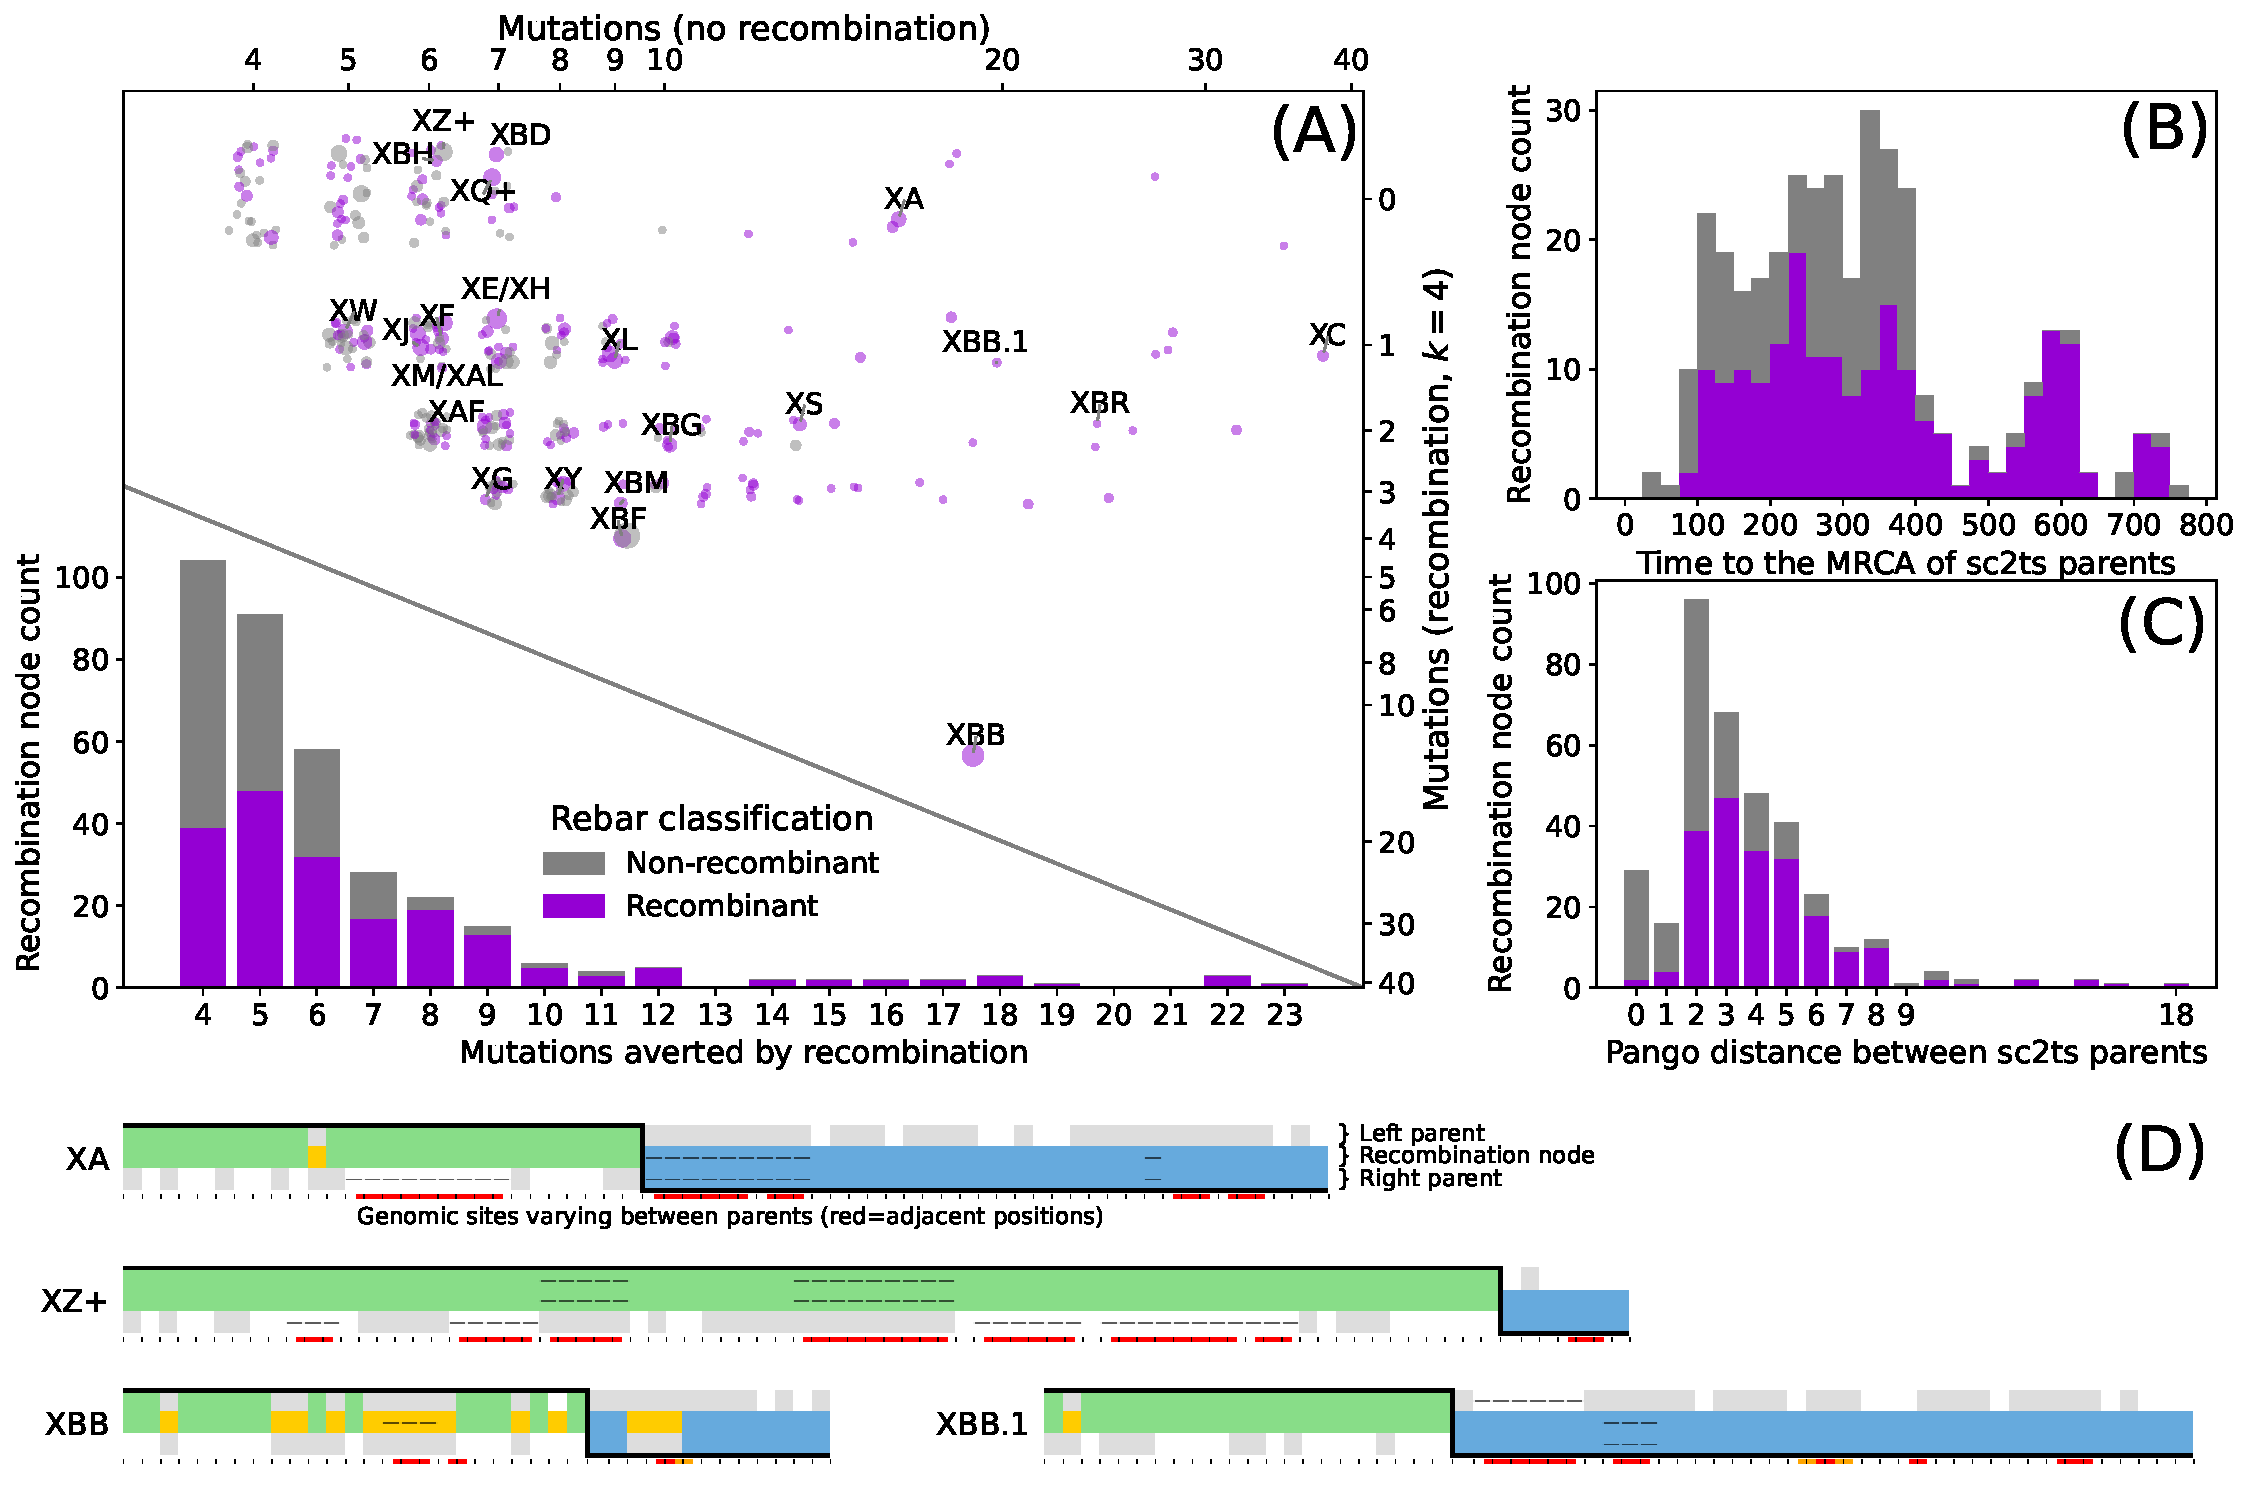
\includegraphics[width=1\linewidth]{fig_recombinant_evidence.pdf}
    \caption{Evidence for recombination in the ARG. All plots show “robust” sc2ts recombination nodes, colored according
to their classification by rebar (recombinant: purple, non-recombinant: gray).
(A) Upper: jittered scatterplot comparing number of mutations when recombination allowed ($y$: right axis)
versus an alternative copying path disallowing recombination ($x$: top axis);
recombination nodes in Table \ref{tab:pango_x_lineages} are labelled, point sizes reflect number of descendants;
Lower: recombination nodes classified by number of mutations averted by allowing recombination (i.e. $x$-$y$).
(B) Distribution of time to the MRCA of the parents of each robust recombination node.
(C) Distribution of the Pango lineage distance between parents.
(D) Copying patterns leading to XA, XBB, XBB.1, and the recombinant origin of XZ+XAC+XAD+XAE+XAP;
each recombination node is a mix of variants matching the left parent (green), the right parent (blue), and de-novo mutations (gold).}
    \label{fig:averted_mutations}
\end{figure}


\subsection*{Recombination breakpoint intervals along the genome}

We explored the spatial distribution of the breakpoint locations of
the “robust” recombination events along the genome, and quantified how precisely breakpoints were localized.
For each event, we computed an interval estimate of its breakpoint location,
using its size as a measure of precision (median, 2,207 bases; STAR Method).

We find an overall preponderance of breakpoint intervals towards the 3’ end of the genome,
particularly at the left boundary of the Spike gene (\ref{fig:landscape}),
consistent with the pattern of excess observed in previous studies \cite{Turakhia2022,Li2024}.
While this might result from a higher recombination rate in this region,
it may also be due to the higher levels of polymorphism in the Spike gene,
allowing recombination endpoints to be estimated more precisely.
Reassuringly, sites having unusually high mutation counts are absent in this region (\ref{fig:landscape}),
which would confound recombination detection.

Furthermore, we find a negative relationship between
breakpoint interval size and the amount of divergence between recombinant parents,
which is measured by time to their MRCA (\ref{fig:landscape}).
When the two parental lineages have diverged for longer periods of time (the rightmost points),
more information becomes available on either side of a breakpoint to pinpoint its location, resulting in shorter intervals.
For instance, the breakpoint intervals tend to be the smallest for events involving recombination
between the deeply divergent Omicron BA.1 and BA.2 sublineages (the red points in \ref{fig:landscape}).

%%% TODO: Old version as placeholder. This figure is not yet finalised.
\begin{figure}[h]
    \centering
    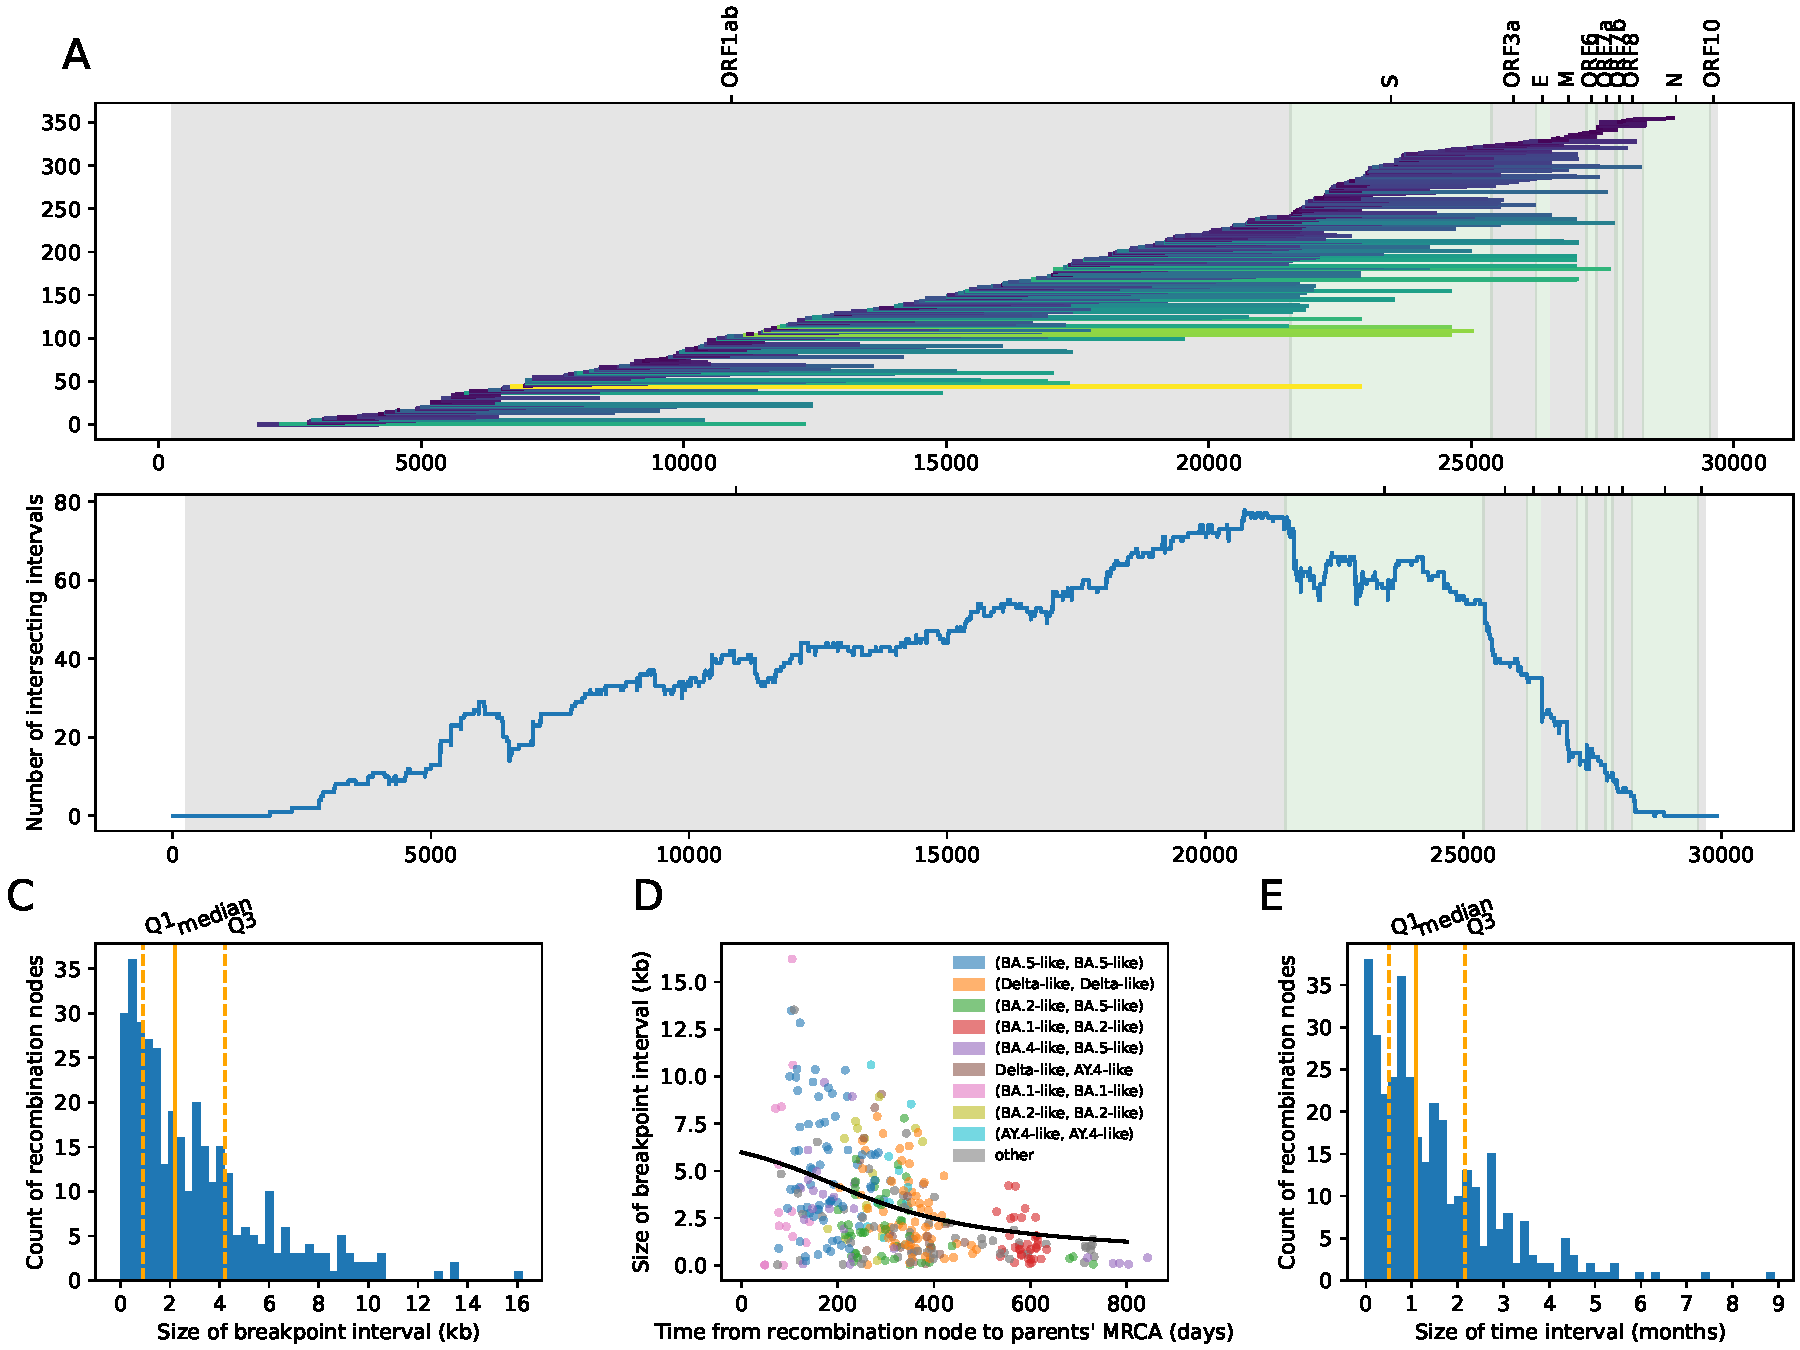
\includegraphics[width=\linewidth]{recombinant_intervals}
    \caption{Recombination intervals. (A) Distribution of the breakpoint
intervals of the 356 ``robust'' recombination events along the genome
(annotated with gene labels on top). Each line represents an interval colored by its size.
(B) Number of overlapping breakpoint intervals.
(C) FIXME Heatmap showing the co-occurrence counts of the parents classified by Scorpio designations.
(D) Relationship between breakpoint interval size and time between the recombination event
and the parental MRCA. The black curve shows the theoretical expected relationship
between these quantities, estimated by minimizing the sum of squared residuals
given a single parameter (the mutation rate) (STAR Methods).}
    \label{fig:landscape}
\end{figure}


\subsection*{Emergence of recombinants over time}

We examined the frequency of emergence of the recombinants over the course of the COVID-19 pandemic (Figure \ref{fig:recombinants_over_time}).
We explored two hypotheses for the timing of recombination.
First, we would expect recombination events to occur more often when case counts are high,
which increases the chance of co-infection within an individual, allowing recombination.
Second, we would expect recombination events to be detected more often when lineage diversity is high,
as this increases the chance that two sufficiently distinct viruses co-infected an individual,
increasing our power to detect recombination.

We used the COVID-19 Data Repository at Johns Hopkins University \cite{Dong2020}
to relate the timing of recombination events with global case numbers.
Case numbers ($n$) were binned by week from January, 2020 to March, 2023 and
sub-divided by the proportion in each Scorpio label inferred within the ARG (shading in \ref{fig:recombinants_over_time}).
These lineages correspond loosely to a group of related lineages within a major VOC in the Viridian dataset.
Alongside the case numbers,
the black curve shows the number of recombinants inferred within each week along the ARG,
focusing on the 356 “robust” events.
Recombination events were inferred more often during the Delta and Omicron waves, when case counts were high.
Overall, the number of recombinant events rose with the global number of cases
(Figure \ref{fig:recombinants_over_time}B; linear regression: $1.0 + 2.7 \; 10^{-7} x$, $p = 1.1 \; 10^{-7}$).
Recombination events also rose with the diversity of lineages in each week
(Figure \ref{fig:recombinants_over_time}C; linear regression: $0.9 + 4.8 x$, $p = 3.4\;10^{-7}$),
measured as the chance that two randomly drawn viruses have different Scorpio designations
($H$, referred to as the “expected heterozygosity”).

We then asked which single measure best explains the number of recombination events inferred each week,
considering $n$, $H$, $n \; H$, $n^2$, $n^2 H$.
We included the squared number of cases each week thinking that it might better predict co-infections.
The best single predictor of recombination events involved the product of cases and expected heterozygosity ($n \; H$),
with an adjusted $R^2$ of 23.7\%.
This measure of case diversity ($n \; H$) explained 49\% more of the variation in recombination events per week
than the next best predictor ($H$, adjusted $R^2$ of 15.9\%).
While consistent with the hypotheses that recombination events occur more often when infection rates are common
and are detected more often when viral diversity is high, we note several sources of uncertainty.
Global case numbers were underreported, particularly during the Delta and Omicron waves \cite{Wang2025}.
Furthermore, there may be substantial uncertainty in the timing of a recombination event,
particularly if these occur in chronically infected individuals (as reported by \cite{Burel2022})
with substantial delays before onward cases are detected.
Finally, the filters that we applied removed all but the most strongly supported recombination events,
although similar conclusions were obtained when all 855 recombinants were considered (STAR Methods).

%%% TODO: Old version as placeholder. This figure is not yet finalised.
\begin{figure}[h]
    \centering
    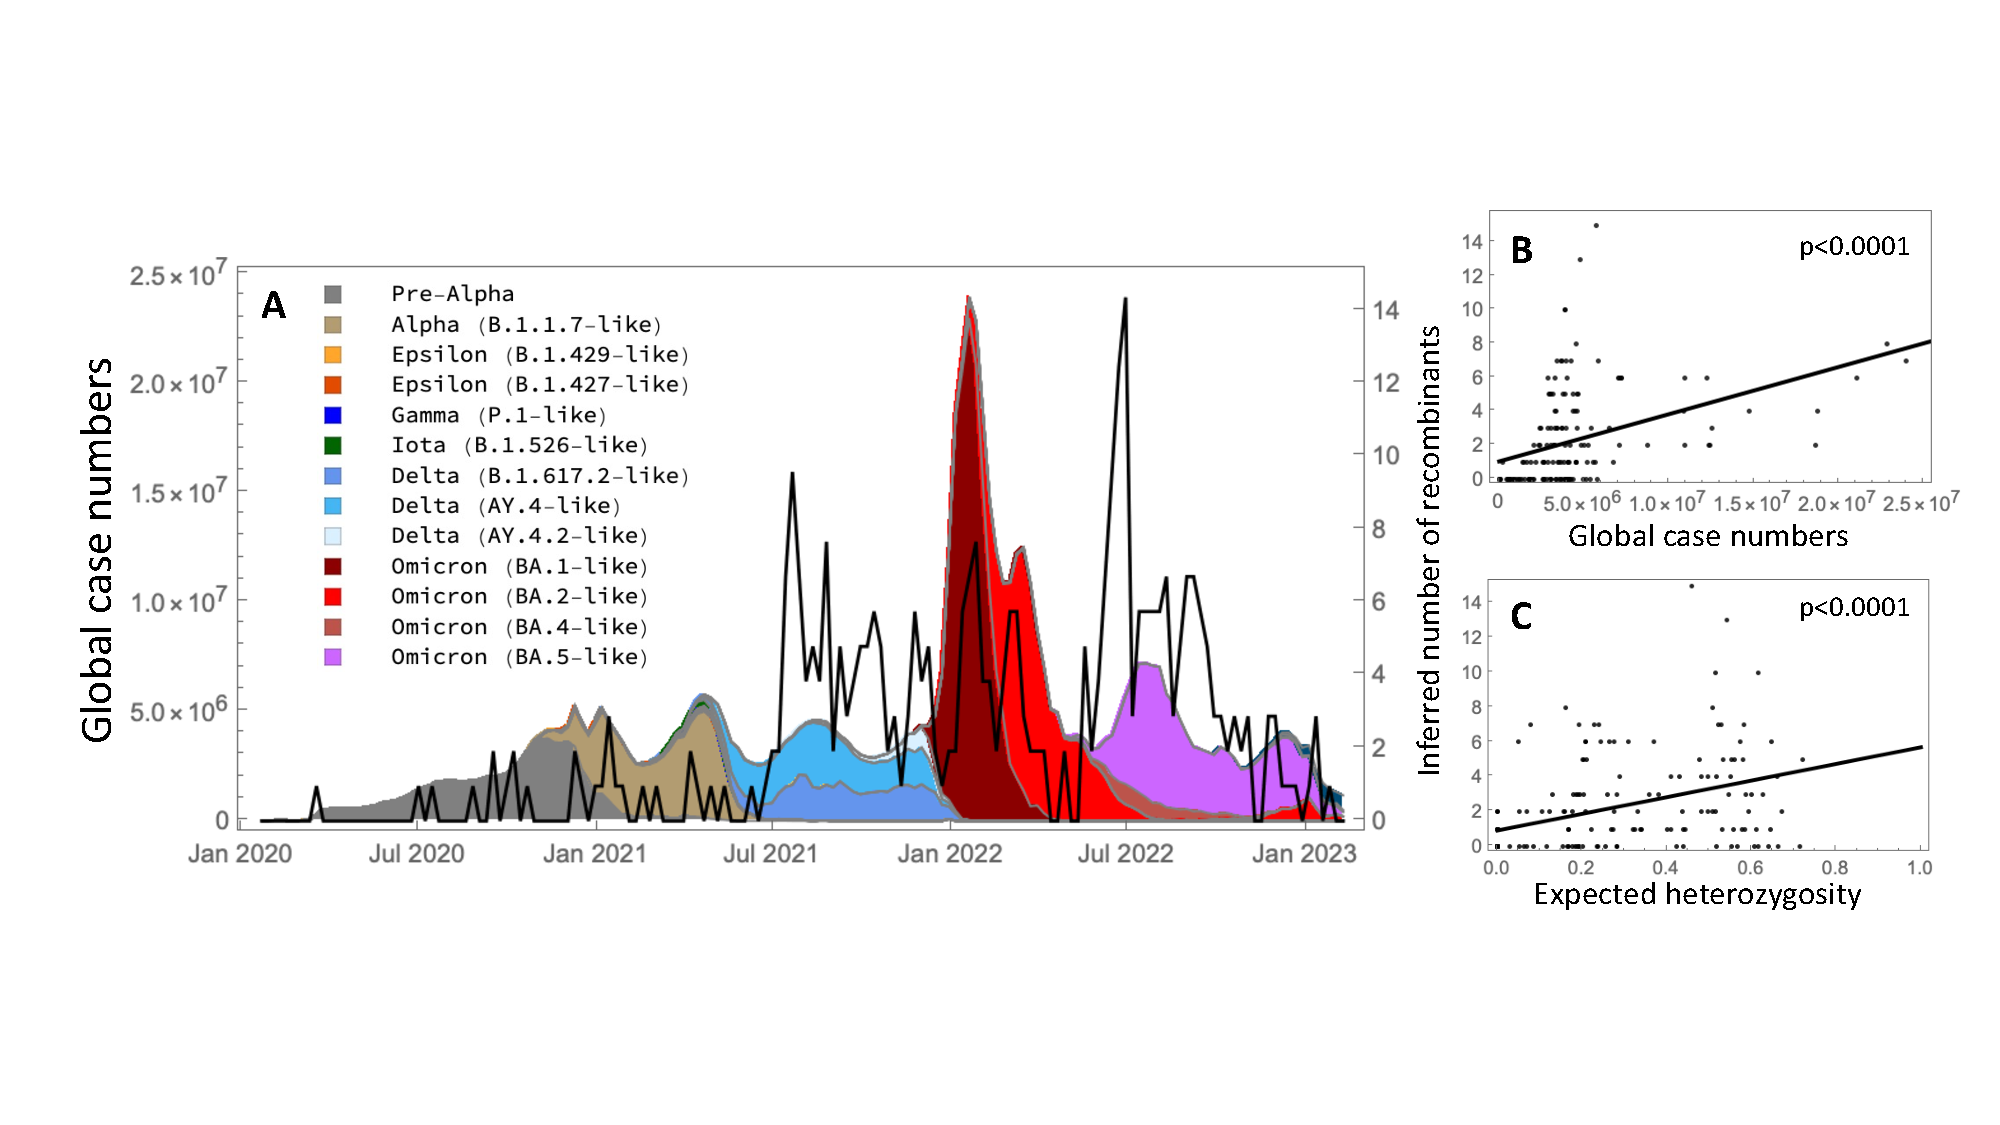
\includegraphics[width=0.85\linewidth]{recombinants_over_time.pdf}
    \caption{Recombination events across the pandemic. (A) Timing of the recombination events (black curve, right y-axis) relative to the global case numbers (\cite{Dong2020}; left y-axis). Cases are color-coded by their Scorpio labels, with the key showing those groupings with $\geq 1,000$ samples in the Viridian dataset. Recombinants more commonly occur (B) in weeks with high case numbers and (C) in weeks with extensive lineage variation, as estimated by high expected heterozygosity; solid lines show fits by linear regression, allowing for non-zero intercepts to account for unknown cases and heterozygosity not captured by the Scorpio labels.}
    \label{fig:recombinants_over_time}
\end{figure}


\subsection*{Efficient inference and analysis of a pandemic-scale ARG}
The COVID-19 pandemic resulted in the collection of viral genome sequence data on an unprecedented scale,
which overwhelmed existing computational approaches,
motivating the rapid development of new methods \cite{Turakhia2021,DeMaio2023,Hinrichs2024}.
Although the computational tools used in phylogenetics and population genetics have historically been largely distinct,
the functionality required largely overlaps.
Sc2ts was built by modifying components of the tskit ARG software ecosystem \cite{Kelleher2019,Ralph2020,Baumdicker2022,Wong2024}
and the VCF Zarr data storage format \cite{Czech2025}
to describe relationships among virus samples, building an ARG over time as data becomes available.
By reusing high-quality and high-performance components of these toolkits,
we could develop the sc2ts inference method itself and
perform all the pandemic-scale analyses in this article with Python code alone and
no compiled languages.

To illustrate the power of these libraries, we provide some examples
in which we compare the Usher and sc2ts intersections in tskit format described earlier.
First, we computed levels of concordance when imputing missing and ambiguous bases in the alignments.
The total aligned dataset for 1,226,587 samples and 27,431 sites shared by the sc2ts and Usher tree sequences
represents 31.34 GB of nucleotide calls.
Of the 80,574,518 missing data calls (Ns) in the alignments,
sc2ts and Usher disagreed in their imputed values for only 56,782 sites (0.07\%).
Additionally, 413,303 calls made use of the IUPAC uncertainty codes.
Of these sc2ts imputed only 77 (0.02\%) incorrectly (i.e., with a base that is not compatible with the ambiguity code).
UShER imputed only 4 calls from this set incorrectly,
reflecting its explicit incorporation of IUPAC uncertainty codes in parsimony calculations.
This computation, performed by co-iterating over the sites in the alignments and the sc2ts and Usher trees,
required 30 lines of Python code and took 2m59s on an intel i7-9700 CPU, with a peak memory usage of about 4.5 GB
(see \cite{Czech2025} for further benchmarks for processing the Viridian data in VCF Zarr format).
Performing this analysis using matUtils would require exporting the full dataset to VCF,
and converting the VCF to FASTA, and then comparing the alignments one-by-one to the source FASTA alignments.
In contrast with matUtils and most phylogenetic software,
which provide a command line interface and suite of predefined operations that typically output text files,
tskit is a Python API (with C and Rust interfaces also supported) which has many advantages \cite{Baumdicker2022}.
As an illustration of the open-ended and efficient nature of the analyses this enables,
we computed the number of polytomies (nodes that have $> 2$ children)
and the maximum number of children per node in the Usher and sc2ts outputs.
In the Usher tree it took 116 ms and 4 lines of code to count polytomies (171,148)
and compute the maximum number of children (5918).
In the sc2ts ARG, it took 385 ms and 6 lines of code to find the maximum number of polytomies (137,001) and
maximum number of children (7708) across all 348 local trees.


\section*{DISCUSSION}

%%% The discussion should explain the significance of the results
%%% and place them into a broader context. Subheadings are permitted.

We present sc2ts, a real-time ARG inference method,
and applied it to build a \~2.48 million-sample pandemic-scale ARG of SARS-CoV-2.
By identifying specific samples as parents,
sc2ts enables more precise interpretation of recombinants than state-of-the-art recombination detection methods,
which find recombinants by matching a given sample to pre-defined population-averaged mutational profiles of Pango lineages.
Sc2ts treats recombination as an integral part of SARS-CoV-2 evolution, in contrast to RIPPLES \cite{Turakhia2022}
which detects recombinants post hoc by searching for unusual branches in a given phylogeny,
inevitably resulting in an incomprehensive representation of SARS-CoV-2 evolution.
Combined with new methods and tools to evaluate evidence for recombination,
sc2ts is a significant technological advance over current methods for the discovery and
analysis of recombinants and efficient inference of SARS-CoV-2 genealogy.

The ARG itself is a useful resource to support future studies of SARS-CoV-2.
Our results show that the ARG captures and unifies important features of SARS-CoV-2 evolution,
which are shown in different studies using different methods, tools, and approaches \cite{Turakhia2022,Bloom2023,Hunt2024}.
The ARG displays remarkable phylogenetic congruence with a state-of-the-art phylogeny built using UShER.
Also, the ARG compactly encodes genetic variation in millions of SARS-CoV-2 genomes,
allowing for convenient and efficient reuse of this valuable dataset
for a variety of evolutionary and genetic analyses beyond those presented here.
We hope that the ARG will spur on new research areas,
in which recombination is naturally and fully accounted for,
and will make an impact comparable to the impact that a recently published human ARG \cite{Wohns2022}
has made on our understanding of human genetic ancestry and demographic past (e.g., REF).

We contribute several novel methods and concepts which may find applications beyond sc2ts.
First, we devise a simplified LS model, which extends the classic concept of parsimony.
In sc2ts, this model allows for accelerated HMM likelihood calculations,
enabling reconstruction of the pandemic-scale ARG presented here.
Existing HMMs used in statistical genetics may be modified in a similar fashion for significant speedup.
Second, we propose the concept of mutations averted by recombination,
which leads to an interpretable quantity to weigh
the support for the hypothesis that a given sample is a recombinant
against the hypothesis that it is a non-recombinant,
considering the sampled genetic diversity in an ARG and a specific HMM.
Third, we propose the concept of HMM cost to identify poorly explained samples
which are either too divergent or have a high number of mutations inconsistent with their collection dates.
Here we use HMM cost to reject time traveling samples,
which no existing phylogenetic method detects and handles during inference
(e.g., in the Viridian UShER phylogeny, parent and child nodes do not necessarily follow time order \cite{Hunt2024}),
resulting in a clean dataset rid of samples with erroneous collection dates that may affect downstream analyses.
Future work may be estimating dates for the suspected time traveling samples using the ARG provided here
and the sc2ts sample matching engine.

Recombination is an important evolutionary force in viruses \cite{Perez-Losada2015},
but has been understudied in part due to a lack of suitable data models, methods, and tools \cite{Neches2020}.
While the methods and tools developed here are tailored for SARS-CoV-2,
they can be extended and adapted for other viruses.
A major advantage of the sc2ts methods and tools is
that they are built on top of the mature software libraries of tskit and VCF-Zarr,
which enable pandemic-scale analyses that can be performed on typical laptops.
Both tskit and VCF-Zarr are developed in Python and leverage the popular PyData ecosystem,
making them highly adaptable for a broad range of applications.
Together with the pandemic-scale ARG, we hope that sc2ts will be highly accessible to many researchers,
enabling and accelerating studies of SARS-CoV-2 for years to come.


\subsection*{Limitations of the study}

%%% A "limitations" or "limitations of the study" subsection in the discussion is encouraged
%%% and may be required for some journals and some article formats.

We close by emphasizing several current limitations and potential directions to improve sc2ts.
First, more stringent filters to exclude false positive recombinants during inference
would obviate post-hoc treatment of these recombinants.
Second, indels carry important phylogenetic signals,
for example, as lineage-defining mutations of Alpha and Delta (REF).
We currently treat multi-base deletions as missing data or multiple independent deletions,
but they are in reality single events.
More sophisticated treatments of multi-base indels in the HMM could help recover additional signals
(and avoid false signals) of recombination.
Third, the current HMM assumes a simplistic mutation model,
which does not account for documented transition-to-transversion rate bias (REF)
and context-dependent variation in mutation rate (REF).
A more realistic mutation model may help improve inference of local genetic relationships in the ARG.
Fourth, an inherent limitation of detecting recombination from sequence data,
which applies to all methods, is that it is impossible to detect events with few (or no) supporting bases,
as these cannot be distinguished from mutation events.
This limitation makes it particularly challenging to detect events near the termini of linear viral genomes.
Fifth, it is challenging to accurately reconstruct global events
when there are regions with poor sampling and jurisdictions with long delays
before sequences become publicly available (REF).
Revisiting the ARG topology periodically
(e.g., rewinding the ARG a month and repeating with samples that became available later)
and better handling of putative recombinants with suspiciously long branches
(e.g., Delta and Omicron BA.2) might improve the accuracy of the genealogy.
Finally, future developments may account for geography in the HMM,
favouring attachment of samples to geographically close lineages.

\newpage


%%%  The following components should appear after the methods.
%%%  For journals using STAR Methods, these components
%%%  should appear immediately after the discussion
%%%  (after any "limitations" or "conclusions" subsection
%%%  within the discussion).

\section*{RESOURCE AVAILABILITY}

%%%  The resource availability section is required
%%%  for all research articles. This component
%%%  has 3 subsections: "lead contact," "materials
%%%  availability," and "data and code availability."
%%%  All 3 subsections must be included, even if no
%%%  unique materials were generated in the study.
%%%  Do not edit or change the names of the subheadings.
%%%  No other subheadings or text are allowed in the
%%%  resource availability section.

\subsection*{Lead contact}

%%%  Authors are required to designate a lead contact,
%%%  who will be responsible for communication with
%%%  the journal before and after publication and is
%%%  the arbiter of disputes, including concerns
%%%  related to reagents or resource sharing. Only
%%%  one author can be named the lead contact, and
%%%  only the lead contact’s information may be
%%%  provided in this section.

Requests for further information and resources should be directed to and will be fulfilled by the lead contact, XX (XX@university.edu).

\subsection*{Materials availability}

%%%  This subsection must include a statement describing
%%%  the availability of newly generated materials
%%%  associated with the paper, including any conditions
%%%  for access. If there are no newly generated materials
%%%  associated with the paper, the statement should
%%%  state this, e.g.: This study did not generate new
%%%  materials.

This study did not generate new materials

\subsection*{Data and code availability}

%%%  All original research papers must include a
%%%  comprehensive and accurate “data and code
%%%  availability” statement within the “resource
%%%  availability” component of the paper before it
%%%  is accepted for publication. These statements
%%%  are structured and consist of three bulleted
%%%  components. Each component must be present.

\begin{itemize}
    \item The ARG and the sequence alignments have been deposited at Zenodo and are publicly available.
    \item All original code has been deposited in GitHub and is publicly available.
    \item Jupyter notebooks to perform the analyses in this paper are available on GitHub.
\end{itemize}


\section*{ACKNOWLEDGMENTS}

%%%  Use this section to acknowledge contributions
%%%  from non-authors and list funding sources,
%%%  including grant numbers.

This work was funded by [FUNDER] via grant [GRANT NO.]. The authors thank all members of the lab for their support.

\section*{AUTHOR CONTRIBUTIONS}

%%%  This component is required for most research papers.
%%%  Mention each individual author with a statement
%%%  outlining the contribution of each author to the work.

Conceptualization, S.C.P. and S.Y.W.;
methodology, A.B., S.C.P., and S.Y.W.;
investigation, M.E., A.N.V., N.A.V., S.C.P., and S.Y.W.;
writing-–original draft, S.C.P. and S.Y.W.;
writing-–review \& editing, S.C.P. and S.Y.W.;
funding acquisition, S.C.P. and S.Y.W.;
resources, M.E.V and C.K.B.;
supervision, A.B., N.L.W., and A.A.D.

\section*{DECLARATION OF INTERESTS}

%%%  This component is required for all articles, even
%%%  if the authors have no competing interests; if
%%%  this is the case, insert "The authors declare no
%%%  competing interests." Please refer to the
%%%  declaration of interests policy:
%%%  https://www.cell.com/declaration-of-interests

S.Y.W. is an employee and shareholder of COMPANY.

\section*{DECLARATION OF GENERATIVE AI AND AI-ASSISTED TECHNOLOGIES}

%%%  If generative AI and AI-assisted technologies
%%%  were used in the writing process, this must
%%%  be disclosed in the paper. This declaration
%%%  does not apply to the use of basic tools for
%%%  checking grammar, spelling, references, etc.
%%%  If you have nothing to disclose, please do not
%%%  include this component.

During the preparation of this work, the author(s) used [NAME OF TOOL OR SERVICE] in order to [REASON].
After using this tool or service, the author(s) reviewed
and edited the content as needed and take(s) full responsibility for the content of the publication.

\section*{SUPPLEMENTAL INFORMATION INDEX}

%%%  Supplemental information must be uploaded as
%%%  separate files. In the main text, please list the
%%%  files to be included in a brief index. For details,
%%%  please review the supplemental information guidelines:

%%%  Journals with STAR Methods:
%%%  https://www.cell.com/STAR-supplemental-information

\begin{description}
  \item Figures S1-SX and their legends in a PDF
  \item Table S1. A descriptive title for an Excel file that was too large to appear in the PDF
\end{description}

% \newpage


% \section*{MAIN FIGURE TITLES AND LEGENDS}

% %%%  At final submission, figure files MUST be
% %%%  provided separately as high-resolution image
% %%%  files. All of the panels for a figure should
% %%%  be in the same file. Figures should have
% %%%  clear labels/file names (Figure 1, Figure 2,
% %%%  etc.).

% %%%  Figure titles and legends should be placed
% %%%  at the end of the main text. You do not
% %%%  need to place the figures, nor their titles
% %%%  and legends, within the main text. While
% %%%  typesetting your article, our team will
% %%%  place each figure in the best location
% %%%  based on the final layout and on your
% %%%  figure citations, e.g., (Figures 1A and 1B).

% %%%  Please review the figure guidelines before
% %%%  submitting your final materials:
% %%%  https://www.cell.com/figureguidelines.

% \noindent\includegraphics[width=0.85\linewidth]{Figure1.jpg}

% \subsection*{Figure 1. A brief title that describes the entire figure without citing specific panels}

% The figure legend can be all one paragraph and describe the images (A), graphs (B), and plots (C), etc., together.
% \newline
% (A) Or each panel or group of panels can be described separately, as shown here and below.
% \newline
% (B) Graph of X, Y, and Z.
% \newline
% (C and D) If panels are grouped like this, please explicitly describe each panel, e.g., “Images showing SEM (C) and TEM (D).”
% \newline
% Please define all scale and error bars, and please review the Cell Press figure guidelines before submission: \href{https://www.cell.com/figureguidelines}{https://www.cell.com/figureguidelines}. Example figure created by Cassie Comeau, Cell Press.

% \newpage

% \section*{MAIN TABLES, INCLUDING TITLES AND LEGENDS}

% %%%  Whenever possible, we encourage you to submit
% %%%  your main-text tables as Microsoft Word documents,
% %%%  using Word's table function. This will ensure
% %%%  the best results during conversion. Tables
% %%%  should be numbered Table 1, Table 2, etc. and
% %%%  should not include subpanels (do not use Table 1A,
% %%%  1B, etc.). Give each table a brief descriptive
% %%%  title. Table legends are optional but encouraged.
% %%%  Footnotes (superscript lowercase letters) should
% %%%  be used where necessary to indicate some feature
% %%%  of the data; please do not use bold, italic,
% %%%  colored text, or shading for this purpose. Use
% %%%  separate cells, not line breaks or spaces, for
% %%%  all discrete data elements. Small embedded
% %%%  graphics with color are OK.

% %%%  Like figures, all tables must be cited within
% %%%  the main text, and our typesetting team will
% %%%  place the tables within the typeset paper at
% %%%  the appropriate locations.


% \subsection*{Table 1. A table with clear organization of data}

% \begin{tabular}{|l | l | l | l|}
%  \hline
%  \textbf{Column 1} & \textbf{Column 2} & \textbf{Column 3} & \textbf{Column 4} \\ [1ex]
%  \hline
%  Row A\textsuperscript{a} & 6 & 87,837 & 787 \\ [1ex]
%  \hline
%  Row B & 7 & 78 & 5,415 \\ [1ex]
%  \hline
%  Row C & 545 & 778 & 7507 \\ [1ex]
%  \hline
%  Row D & 545 & 18,744 & 7,560 \\ [1ex]
%  \hline
%  Row E & 88 & 788 & 6,344 \\ [1ex]
%  \hline
% \end{tabular}

% \bigskip

% The table legend (optional) follows the table itself.
% The legend should be used to provide additional info that relates to the table as a whole.

% \textsuperscript{a}Footnotes can be used to provide additional info on specific content within the table,
% such as this footnote to the first row (row A). Do not use footnotes in the table title.

% \textsuperscript{b}More footnotes

\newpage

%%%  REFERENCES: As of 2023, all Cell Press journals
%%%  use Numbered (AMA) style. We recommend placing
%%%  your references in the included "references.bib"
%%%  file.


\bibliography{references}



\bigskip

%%%  In your References, please include only articles
%%%  that are published (online publication and
%%%  preprint servers are OK). Unpublished data,
%%%  submitted and/or accepted manuscripts, abstracts,
%%%  and personal communications should be cited within
%%%  the text only ("unpublished data," "data not
%%%  shown," "Alice Smith, personal communication")
%%%  and not included in the references list. Personal
%%%  communication should be documented by a letter
%%%  of permission. Whenever possible, please make
%%%  sure your .bib file has the complete author lists
%%%  for each item (at minimum, the first 11 authors
%%%  listed).

\newpage






%%% All Cell Press \textbf{life and medical science} journals, and the multidisciplinary journal \textbf{iScience},
%%% use the \textbf{\href{https://www.cell.com/star-authors-guide}{STAR Methods}} format for reporting materials and methods.

%%% If you are publishing in a STAR Methods journal, please refer to the appropriate guide for authors:
%%% Cell authors should download the guide https://www.cell.com/pb-assets/journals/research/cell/methods/Methods_Guide_Cell-1678470557763.pdf.


\section*{STAR METHODS}

%%%  The STAR Methods should appear in your main
%%%  manuscript file after the figure legends, main
%%%  table(s) and table legend(s).

\subsection*{Key resources table}

\textit{To create the KRT, please use the \href{https://star-methods.com}{KRT webform} or the \href{http://www.cell.com/pb-assets/journals/research/cell/methods/table-template1.docx}{Word template} and upload this file separately.}

\subsection*{Method details}

%%%  Please provide precise details of all the
%%%  procedures in the paper (behavioral task,
%%%  generation of reagents, biological assays,
%%%  modeling, etc.) such that it is clear how,
%%%  when, where, and why procedures were
%%%  performed. We encourage authors to provide
%%%  information related to the experimental
%%%  design as suggested by NIH and ARRIVE
%%%  guidelines (e.g., information about
%%%  replicates, randomization, blinding, sample
%%%  size estimation, and the criteria for
%%%  inclusion and exclusion of any data or
%%%  subjects).

\subsubsection*{Description of sc2ts}

Sc2ts (pronounced “scoots”, optionally)
is a method for inferring Ancestral Recombination Graphs (ARGs)
from densely sampled genome sequence data in real time,
in which recombination occurs at a low but significant rate.
The basic idea is to incrementally update an ARG regularly
with the sequences collected since the previous batch \ref{fig:methodology}.
We used daily batches for SARS-CoV-2,
and use days as the time interval for clarity in what follows.
The first step is to find likely “copying paths” under the Li and Stephens (LS) model \cite{Li2003}
for each sequence in the daily batch to the current ARG.
These copying paths will mostly consist of a new sample sequence copying
from a node in the ARG with a small number of mutations,
and often many samples from a daily batch will copy from the same ARG node.
The second step is then to “resolve” these implied polytomies
by using a standard neighbor-joining algorithm \cite{Saitou1987}.
This greedy update strategy inevitably leads to unparsimonious topologies,
and the third step is to then increase the overall parsimony of the inferred ARG
by making some simple topological updates.
Recombination is inferred as an integral and ongoing part of this process,
requiring only a few additional steps to facilitate later analysis.
The result of inference for a given day is then a genealogy recording genetic inheritance
as well as mutation and recombination events
for all of the samples added to the ARG up to that day.


\subsubsection*{Ancestral Recombination Graphs}

%%% This paragraph needs to be rewritten.
Originally introduced (Griffiths, 1991; Griffiths and Marjoram, 1997)
to define an alternative formulation of the coalescent with recombination (Hudson, 1983),
the term “Ancestral Recombination Graph” has come to be used
more generally to describe not just realizations of the model,
but any recombinant genetic ancestry (Minichiello and Durbin, 2006).
While there is some subtlety in the details \cite{Wong2024},
we can think of an ARG as being any graph
that encodes the reticulate genetic genealogy of a sample of sequences
under the influence of recombination.

The “succinct tree sequence” (STS) is an ARG data structure
that is both general (in terms of the types of ancestry that can be described)
and computationally efficient \cite{Wong2024}.
Initially developed to facilitate large-scale coalescent simulations \cite{Kelleher2016},
STS has been extended and applied to
forward-time simulations \cite{Kelleher2018,Haller2019},
calculation of population genetics statistics \cite{Ralph2020} and
ARG inference \cite{Kelleher2019,Wohns2022}.
The STS is based on a simple tabular representation,
which defines a set of nodes, edges, sites and mutations.
A node represents a particular genome, which may be an observed sample or an inferred genetic ancestor.
The genetic inheritance between a pair of nodes along a segment of genome
is defined by the edge ($l$, $r$, $p$, $c$),
which states that child node $c$ inherited its genome from parent node $p$
from left coordinate $l$ to right coordinate $r$.
A site defines a position on the genome and the ancestral state (allele) at that site.
A mutation records the site and node IDs where a mutation occurs and the derived state (allele).

Given the node, edge, site and mutation tables,
we can efficiently construct the local genealogical trees along the genome (arising from recombination)
and perform a range of calculations efficiently
by reasoning about the differences between these local trees \cite{Kelleher2016,Ralph2020}.
These algorithms have led to performance increases of several orders of magnitude over
the state-of-the-art in a range of applications \cite{Kelleher2016,Kelleher2018,Kelleher2019,Ralph2020,Baumdicker2022}.
The STS encoding is also very concise, allowing, for example,
for millions of complete human genomes to be stored in a few GB of space \cite{Kelleher2019},
and so it is particularly well suited to representing large SARS-CoV-2 genealogies.

The SARS-CoV-2 ARGs inferred using sc2ts can be conveniently and efficiently analyzed
using the mature and feature-rich tskit library \cite{Kelleher2018,Ralph2020}.
Tskit is widely used in population genetics, and has been incorporated into many downstream applications
(e.g., \cite{Haller2019,Speidel2019,TerasakiHart2021,Fan2022,Korfmann2022,Mahmoudi2022,Petr2022,Rasmussen2022,Zhang2023}).


\subsubsection*{Li and Stephens haplotype-copying model}

LS model \cite{Li2003} is an approximation of the coalescent with recombination
that captures many of the key features of the joint processes of mutation and recombination.
It is widely used in a range of applications in population genetics, including ARG inference \cite{Kelleher2019,Gunnarsson2024}.
The LS model is an HMM that models a focal genome as a sequence of nucleotides (i.e. the observed states),
which are probabilistically emitted as an imperfect mosaic of a set of genomes in a reference panel (i.e., the hidden states).
The process of switching between the genomes in the reference panel is governed by a transition matrix,
and mismatches between a focal genome and a genome of the reference panel (from which it is “copied”) are permitted as emissions.

In the original formulation of the LS model (see Appendix S1 of \cite{Li2003}),
the probability of switching between the hidden states (i.e., genomes in a reference panel)
when going from one site to the next is dependent on
(1) the rate of recombination between the sites and
(2) the number of genomes in the reference panel ($n$).
Sc2ts uses the same formulation except that n is set to 1.
This special case of the LS model leads to an intuitive interpretation of the ratio
between the probability of switching and the probability of mismatch:
When considering only two copying paths, the path having k mismatches
and the other path having one switch but no mismatch are equally probable.
We call this parameter k the “recombination penalty”.
This parameter thus allows us to adjust the relative importance of recombination and mutation
when finding the best explanation for a given sample.
For simplicity, we assume that any single base mutation causing a mismatch is equally probable,
ignoring transition-transversion biases and variation of mutation rate along the genome.
As data sampling was dense for SARS-CoV-2, this assumption was considered tolerable.

In our early attempts to build ARGs, we explored using several values of $k$.
We ran sc2ts with $k$ set to 3, 4, and 5 on the samples collected in 2020 \cite{Zhan2023}(REF).
We would expect that a good value for $k$ should lead to parsimonious ARGs
that capture plausible recombination events without incurring too many mutations, particularly reversions.
A value of $k$ too low could result in many artifactual recombination events,
whereas a value of $k$ too high could miss many genuine recombination events.
We found that ARGs built with $k$ set to 3 contained many dubious recombination events,
but ARGs built with $k$ set to 5 failed
to include the well supported recombination events documented in a previous study \cite{Jackson2021}.
Hence, we decided to use $k$ set to 4 to infer the final ARG described in this study.

A Viterbi algorithm can be used to find the most likely “copying path” of a focal sample
through a reference panel of samples under the LS model.
Specifically, sc2ts uses a Viterbi algorithm modified to operate on STS,
which was originally developed to build genome-wide human genealogies
and is capable of scaling to biobank-scale datasets \cite{Kelleher2019}.
Using this Viterbi algorithm, sc2ts deterministically infers the copying path of a sample
collected on a certain date through the samples collected on earlier dates in a given ARG.


\subsubsection*{Accelerating sample matching}

The SARS-CoV-2 sequences were determined from samples collected densely in time.
SARS-CoV-2 phylogenies have low phylogenetic signals due to high sampling frequency
(such that sampling and transmission outpace nucleotide substitution).
Therefore, most samples can be explained by a small number of mutations.
Leveraging this property of the dataset, we developed a likelihood-thresholding strategy
to avoid needing to compute the likelihood of all possible copying paths through an ARG for every single sample.
%%% TODO: This needs to be explained.

Furthermore, to avoid performing redundant HMM matching on identical samples, new samples
which were exactly matched to a (sample or non-sample) node in the ARG were not added immediately.
Instead, the copying paths of these samples were recorded,
and the samples were eventually added back to the ARG in a post-processing step.


\subsubsection*{Tree inference from daily sample clusters}

With tens of thousands of samples being added to the ARG per day,
there are often clusters of hundreds of sequences attaching to the same node
(or more generally, the same recombinant path).
While some of these samples will require no extra mutations
(as they are identical to the attachment node),
in general there will be complex patterns of shared mutations among the samples
reflecting their evolutionary relationships.
A natural way to infer these within-cluster evolutionary relationships
is to use standard tree-building algorithms.
We can infer a plausible phylogeny relating the samples in a cluster
independently of the other samples in a daily batch
and then attach the phylogeny (and mutations) to the ARG at the node
identified by the LS model.

Sc2ts builds a local phylogeny relating the samples in each cluster as follows.
First, it infers a tree using a standard neighbor-joining algorithm \cite{Saitou1987}.
Then, mutations are mapped back onto it using the Fitch-Hartigan parsimony algorithm \cite{Fitch1971,Hartigan1973}.
Finally, the resulting tree is added to the ARG at an attachment node
and the ARG is locally modified using heuristics to improve parsimony (Figure SX).
For a recombinant, the attachment node is the inserted (non-sample) recombination node associated with it.
For a non-recombinant, it is the common parent in the copying paths of the samples.


\subsubsection*{Handling outlier samples}

Although we expected that most samples can be explained by a small number of mutations in the ARG,
we observed two types of outlier samples which had unusually high numbers of mutations:
(1) “time travelers” and (2) “saltation” lineages.
Time traveling samples are caused by errors in their collection dates.
For example, if a sample is actually collected 10 months after its reported collection date,
then 20 mutations (instead of, say, 0 or 1) are needed to explain it
using the ARG available on its collection date,
assuming a substitution rate of 2 events per genome per month.
Samples from “saltation” lineages (particularly the major VOCs) are characterized
by high numbers of mutations by the time of their detection.
Both types of outlier samples are poorly fit to the ARG when they appear on their collection dates.
To handle these outlier samples, we introduce three mechanisms:
(1) HMM cost-based rejection,
(2) retrospective sample grouping, and
(3) unconditional seeding.

First, we introduce a rejection mechanism to prevent samples
that are generally poorly explained by the ARG
using the LS model parameterised by a specific value for the recombination penalty ($k$).
For each sample, an HMM cost is calculated based on the number of switches and mismatches
in its most likely copying path under the LS model:
The sum of the penalty cost for the switches ($k$)
and the penalty cost of the mismatches (implicitly, equal to one).
To build the ARG described here, we used $k$ of 4 and a maximum HMM cost of 7.
This combination of parameter values rejected samples which have no switch
but 8 mismatches as well as samples which have one switch and 4 mismatches.
It is important to note that this does not necessarily mean
that samples with more than 8 mismatches
or samples with two or more switches cannot be incorporated into the ARG.
Such samples can be added back using a separate mechanism (see below).
We find that although it effectively removes time travelers with poor sample support (e.g. singletons),
the mechanism can filter samples too aggressively.
For example, in preliminary ARGs, it led to exclusion of major saltation VOCs (e.g. Alpha).

Second, to prevent exclusion of the important saltation VOCs
(and less important but well supported poorly-fit lineages),
we introduce “retrospective sample grouping”.
The idea is to gather evidence for a lineage within a time window rather than on a single day.
After adding a batch of samples, the samples initially rejected on their collection dates
due to high HMM costs are reconsidered for attachment to the ARG if
(a) they are collected within a retrospective time window (the past 7 days);
(b) they have identical copying paths; and
(c) they have shared immediate reversions
(attaching a new sample to the top or the bottom of a long branch).
Sample groups satisfying these criteria are attached to the ARG if
(a) they have at least 10 samples;
(b) they are collected on at least 3 different dates
(to avoid adding batches of time travelers having the same collection date); and
(c) they have at least two shared “non-immediate” reversions
(so as to prevent unrelated time travelers from being grouped together).
Furthermore, phylogenetic tree quality metrics are used to preclude groups of samples
that are unlikely to be closely related.
Specifically, the tree of a sample group was excluded if
(a) it has more than two recurrent mutations or
(b) it has more than 5 mutations per sample on average.

Retrospective sample grouping successfully captured most saltation lineages,
but integrating Delta and Omicron into the ARG required further manual intervention.
To ensure that Delta and Omicron are added, we introduce a third mechanism, “unconditional seeding”.
The idea is to choose suitable samples belonging to each VOC,
and attach them to the ARG unconditionally (i.e. without filtering using HMM cost).
We sought “seed” samples for Delta, Omicron BA.1, and BA.2.
For Delta, we used two sets of seeds:
(1) 8 samples assigned to B.1.617.2, and
(2) 9 additional samples assigned to its sibling lineage B.1.617.1.
Specifically, these samples are the earliest samples present in the Viridian v04 dataset
that were used for the designation of the VOCs.
For Omicron BA.1 and BA.2, we used SRR17041376 and SRR17461792, respectively.
We chose SRR17041376 (a sample dated 2021-11-12 from South Africa)
as the BA.1 seed (https://github.com/jeromekelleher/sc2ts-paper/issues/264),
as it could be well explained as as a non-recombinant given the ARG available on its collection date.
For BA.2, we chose SRR17461792 (dated 2021-11-27 from South Africa),
which is the earliest BA.2 sample present in the Viridian v04 dataset.
It is dated later than SRR17041376 (the BA.1 seed),
allowing time for the BA.1 lineage to accumulate enough sampled descendants
and to get established in the ARG.
For the full list of seeds,
see
\url{https://github.com/jeromekelleher/sc2ts-paper/blob/main/inference/viridian\_config.toml}

In practice, it is difficult to find optimal seeds for saltation lineages,
which ideally would require no reversion to be added to the ARG
and to which sampled descendents would be added with no reversion.
Considering poor early sampling and the presence of time travellers for Delta, Omicron BA.1, and BA.2,
using suboptimal seeds is likely the best that we can do in practice.
The consequence is that there would be some reversions leading to the samples attached to the seed(s).
Nevertheless, it is a better alternative to not using seeds,
as there would be far more reversions (as seen in preliminary ARGs built without seeding).
The caveat of taking this approach is that one must be more careful
when analysing the samples around the seed(s) in the ARG.


\subsubsection*{Data preprocessing}

In this study, we used the SARS-CoV-2 sequences reassembled in a recent study \cite{Hunt2024}
using an amplicon-aware assembly method (named “Viridian”).
The Viridian sequences contain far fewer artifacts compared to their publicly deposited counterparts on GenBank.
Consequently, phylogenetic tree inference using the Viridian data led to more parsimonious phylogenies,
as seen by a large reduction in the number of likely artifactual reversions \cite{Hunt2024}.

We downloaded 4,484,157 Viridian sequences obtained
from samples collected from January, 2020 to March, 2023 (“batch 1”).
We aligned each sequence to the Wuhan-Hu-1 reference sequence (MN908947.3) using MAFFT v7.525 \cite{Katoh2013},
with the option ‘--keeplength’ to retain the reference coordinate system, discarding insertions.
We converted the MAFFT alignments and all sample metadata to VCF Zarr format \cite{Czech2025},
which are available for download on Zenodo (URL).

Prior to ARG inference, we preprocessed the remaining sequences as follows.
We treated low-quality bases (represented by Ns), gaps and ambiguous characters in the sequences as missing data.
When encoded as missing data, the bases do not inform sample matching (see “The Li and Stephens model”).

During inference, we filtered out the samples with low-quality sequences and low-precision sampling dates.
We kept the quality check-passing sequences used to infer the Viridian UShER phylogeny \cite{Hunt2024}.
We skipped low-quality sequences that had more than 500 missing sites
(except when building the “base” ARG, when the maximum number of allowed missing bases was set to 10,000 instead).
We also skipped ~40,000 samples which had a collection date of December 31, 2020.
The sampling frequency of this date is alarmingly high compared to other dates (at most 15,000 samples per day).
We suspect that this batch of samples might be unusually enriched for wrong collection dates,
likely due to arbitrary assignment of the originally reported collection date of “2020” to be “31-12-2020”.
Furthermore, manual checking (by cross-referencing the ENA and COG-UK Mutation Explorer)
confirmed that some of the samples were not collected in 2020.

Sites which are enriched for systematic sequencing errors or frequently experience homoplasy
can cause artifactual signals of recombination (REF).
The bioinformatics community has identified and curated a set of problematic sites
that are recommended to be excluded before phylogenetic inference (REF).
Here we assembled a bespoke set of such problematic sites
using the information in the Viridian sequences.
To do so, we first built a preliminary ARG from the samples collected up to June 30, 2021,
without any site masking.
Then, we identified the top 100 sites which had the highest mutation counts in the ARG (URL).
Only six of these sites overlapped with the “Problematic Sites”
downloaded from the UCSC Genome Browser website (URL),
which did not have a high number of mutations in the preliminary ARG.
To infer the final ARG, we masked the problematic sites
in our custom set
\url{https://github.com/jeromekelleher/sc2ts-paper/blob/main/inference/viridian\_config.toml}.

\subsubsection*{Reconstructing a pandemic-scale ARG}

%%% TODO: Much of this needs to be rewritten once the post-processing pipeline is finalised.
Using sc2ts, we reconstructed the ARG presented here in three stages:
(1) initialization, (2) extension, and (3) post-processing.

First, we initialized a base ARG.
We added the Wuhan-Hu-1 reference sample (MN908947.3) as the root node, dated December 8, 2019.
Then, we ran sc2ts unconditionally (i.e., without excluding samples by HMM cost) up to March 01, 2020 (inclusive).
This step is necessary to accumulate sufficient genetic diversity in the ARG
for subsequent sample matching and attachment in the next stage.

Second, we extended the base ARG by adding batches of samples collected on and after March 02, 2020.
Sample filtering, HMM cost-based rejection, and retrospective sample grouping, as described above,
are in full effect during this stage.

Finally, we performed the following post-processing steps
to modify certain non-topological properties of the ARG or
to enrich the ARG with additional information:
1. Moving mutations around recombinants? TODO
2. Adjusting recombination breakpoints. XX.
3. Mapping multi-base deletions. Multi-base deletions are challenging to handle, as they violate the Markov property of the HMM. In our ARG, insertions are deleted regions that acquire nucleotides (not necessarily the same nucleotides) without altering the genome length, because we discarded length-changing insertions when preprocessing the aligned sequences. We treated multi-base indels as multiple separate mutations in the HMM. We mapped them back onto the inferred ARG as single events.
4. Mapping mutations at masked sites. XX.
5. Adding exactly matched samples. During sample matching, samples identical to node(s) in a given ARG were not added to the ARG. Instead, after inference, we simply added the nodes to the ARG using the saved matching results. This allowed for computational savings, as it kept the number of possible parents available for matching to a minimum.
6. Estimating non-sample node ages. The ages of the inserted non-sample nodes (the nodes in the local trees and the recombination nodes) were initially assigned to arbitrarily determined values. We ran \textit{tsdate} (“variational gamma”, version XX; \cite{Wohns2022} Pope et al., 2025) on the ARG to adjust the ages of these nodes, while fixing the ages of the sample nodes to the reported collection times (defined as fractional years before the collection date of the last sample added to the ARG, which is February 20, 2025 in the ARG described in this study).
7. Assigning Pango lineages to non-sample nodes.


\subsubsection*{Comparing phylogenetic backbones}

We used Pango lineage designations to select \textit{representative} samples
for the majority of the 2026 Pango lineages in the ARG.
We first identify an "origination node" for a focal Pango lineage,
defined as the oldest internal node in the ARG
whose descendants in any tree include more than 50\% of the Pango samples of the focal type,
and where the internal node is itself designated as the focal Pango.
The representative sample is then chosen as the oldest sample under the origination node
whose own descendants (if any) are entirely of the focal Pango type.
We simplify the ARG to include only the representative samples,
resulting in an intermediate ARG of 1867 samples,
then additionally remove internal samples,
known recombinants (i.e. the Pango Xs) and three "singleton recombinant samples"
in which a single Pango lineage appears immediately below a recombination node.
This results in a simplified ARG of 1667 samples, each with a different Pango designation.

We compare topology in the simplified ARG against the UShER tree, built from the Viridian dataset.
To remove time traveling samples from the UShER tree,
we reduce it to 2475419 samples shared with the main sc2ts ARG
and date the internal nodes by running tsdate,
with no rescaling and the root node constrained to the established date of the UShER root (2020-01-16).
To compare against the ARG, we simplify this UShER tree down to the 1667 representative ARG samples.

The simplified ARG contains four single-breakpoint recombination nodes,
corresponding to the origins of Delta, BA.2, BA.5, and a further BA.2 recombinant
which we deem artifactual by our standard criteria
and treat as non-recombinant for the purposes of plotting
(the breakpoint is on the far right at position 27382,
and supported by only 4 distinguishing sites / 3 loci).
To reduce plot density, we consider only those Pango lineages with fewer than 10 samples,
and extract non-recombinant structures from the ARG
by creating a "base tree" of 535 Pangos (i.e. excluding all descendants of Delta, BA.2, and BA.5),
a Delta subtree of 160 Pangos,
a BA.2 subtree of 151 sample (excluding BA.5 descendants) and
a BA.5 subtree of 251 samples.
Figure SX shows each of these trees compared against the equivalent dated UShER topology,
with the left and right parents of Delta and BA.2 highlighted in the base tree.
The order of tips in the two trees was chosen to reduce tangling,
as calculated using the NeighborNet algorithm from Dendroscope \cite{Scornavacca2011,Huson2012},
with tanglegrams plotted using the SVG outputting facility built into tskit.
The entire pipeline is saved as a notebook at URL (?).

The majority of resolvable nodes, including most high-level Scorpio groupings,
are shared between the ARG and the UShER tree (magenta nodes).
In the few cases where the trees differ, this is often in terms of degree of resolution of polytomies.
In these cases, sometimes the sc2ts ARG shows greater resolution,
as in the base of the BA.2 subtree, and
sometimes the UShER tree shows greater resolution, as in BA.2.9.


\subsubsection*{Counting supporting loci for recombinant parents}
When counting such loci, we considered nearly adjacent sites (separated by at most three bases) as single loci,
to avoid over-counting support from correlated loci, which would lead to artificial signals of recombination.
Also, when counting supporting loci for a focal parent,
we penalized loci where the character(s) in the recombinant matches that in the non-focal parent but not in the focal parent.


\subsubsection*{Calculating Pango lineage distance using pangonet}
We define a “pseudo-phylogenetic” distance to quantify the divergence between two Pango lineages.
The idea is to count the number of edges separating two given Pango lineages in a “pseudo-phylogeny”
which relates all the designated Pango lineages.
To construct this pseudo-phylogeny, we used \textit{pangonet},
which mines the information on the Pango lineages in the ``alias\_key.json''
and ``lineage\_notes.txt'' files
from the Pango designation issues (https://github.com/cov-lineages/pango-designation).
If two Pango lineages are siblings in the pseudo-phylogeny,
the distance is defined as the sum of the number of edges from each lineage to their MRCA;
if they are non-siblings (i.e. one Pango is a descendant of the other),
the distance is defined as the number of edges separating them;
if they are identical, the distance is defined as zero.


\subsection*{Quantification and statistical analysis}

%%%  Please describe here all statistical analysis
%%%  and software used. We ask authors to indicate
%%%  in this component where all of the statistical
%%%  details of experiments can be found (e.g., in
%%%  the figure legends, figures, results, etc.),
%%%  including the statistical tests used, exact
%%%  value of n, what n represents (e.g., number
%%%  of animals, number of cells, etc.), definition
%%%  of center, and dispersion and precision
%%%  measures (e.g., mean, median, SD, SEM, confidence
%%%  intervals). Also, please summarize in this
%%%  component how significance was defined, the
%%%  statistical methods used to determine strategies
%%%  for randomization and/or stratification, sample
%%%  size estimation, and inclusion and exclusion
%%%  of any data or subjects, as well as any methods
%%%  used to determine whether the data met
%%%  assumptions of the statistical approach.

\subsubsection*{Estimating interval lengths}
Recombination intervals are imprecise
when the recombining parents are identical in sequence at sites spanning the breakpoint.
Here we estimate the interval lengths expected around a breakpoint,
given a genome-wide mutation rate $\mu$,
total time between two samples ($T$), and
sufficient support to detect the recombination event.
If a breakpoint occurs a fraction $P$ along a genome of length $L$ and
$k$ mutations have occurred to the left of the breakpoint,
then we expect the nearest mutation to occur $P L / (k + 1)$ bases to the left.
If we require $n$ mutations on both sides of the breakpoint,
we can calculate the expected value of the interval to the left by summing across a Poisson-distributed number of mutations,
conditioned on having at least $n$ mutations:

\[I_{left} = \frac{L}{n T \mu} \frac{\Gamma(1+n) - \Gamma(1+n, P T \mu)}{\Gamma(n) - \Gamma(n, P T \mu)}\]

A similar result holds for the right interval ($I_{right}$), but with $P$ replaced with $1–P$.
Summing the two intervals ($I_{left}+I_{right}$) gives the expected interval length.
As detectable recombination events are nearer the center of the chromosome, we use $P=½$ in Figure X.


\subsubsection*{Analyzing global case counts}
To explore the timing of emergence of recombinants,
case count data were downloaded from
the COVID-19 Data Repository by the Center for Systems Science and Engineering (CSSE)
at Johns Hopkins University \cite{Dong2020} and binned by week from January, 2020 to March, 2023.
The proportion of each lineage $i$ in each week ($p_i$) was then inferred
from the Scorpio designation at each node within the ARG for that week.
Genetic variation was measured as the “expected heterozygosity” across lineages,
which is the chance that two lineages chosen at random
from that week had different Scorpio designations ($\sum_{i} \sum_{j>i} 2 p_i p_j$).
The linear regression models reported in \textbf{Figure} \ref{fig:recombinants_over_time} allowed for a non-zero intercept,
because there may be unreported cases even without any reported cases.
The slopes were highly significant, and
the p-values were confirmed by randomly permuting the predictor variable 10,000 times.
ANOVAs were conducted to determine which single predictor ($n$, $H$, $n \; H$, $n^2$, $n^2 H$) explained the most variation in recombination events by week.
These statistical tests and graphics were conducted in \textit{Mathematica} 14.2 (Wolfram 2024) and available at GITHUB LINK.

In addition to the analysis of the 356 “robust” recombination events with a minimum of four nucleotides supporting each parent,
we analyzed the relationship between the full set of 855 recombinants and case numbers.
These additional recombinants occurred disproportionately during the Delta and first Omicron wave (July, 2021 to February, 2022).
Again, the number of recombinant events rose with the global number of cases
(linear regression: $3.1 + 5.3 \; 10^{-7} x$, $p = 0.0006$)
and with the diversity of lineages in each week
(linear regression: $0.42 + 18.3 x$, $p = 2 \; 10^{-12}$).
The single best predictor of recombination events among the predictors tested ($n$, $H$, $n \; H$, $n^2$, $n^2 H$)
was again the product of cases and diversity ($n \; H$),
with an adjusted $R^2$ of 26.9\%,
although this was now followed closely by expected heterozygosity on its own ($H$),
with an adjusted $R^2$ of 26.5\%.
Thus, similar conclusions are reached with either dataset,
although filtering the recombination events to the 356 with better support revealed a stronger relationship with case numbers.


\subsection*{Additional resources}

%%%  Please provide links to websites that provide
%%%  further information relevant to the study
%%%  (e.g., protocol download, troubleshooting
%%%  forum, etc.). Clinical trial registry numbers
%%%  and links should also be placed here. Please
%%%  briefly describe the resource and its
%%%  relevance for the paper. Please report this
%%%  information as: “Description: URL.”

Cell.com homepage: https://www.cell.com
\newline Templates for Cell Press authors: https://www.cell.com/article-templates

%%%  ADDITIONAL MANUSCRIPT COMPONENTS:

%%%  Depending on the journal and the article
%%%  type, you may be asked to upload the
%%%  following as separate files: graphical
%%%  abstract, highlights, eTOC blurb (In
%%%  Brief), and/or other article components
%%%  such as a "bigger picture" statement.
%%%  These items are typically not required for
%%%  initial submissions. Please refer to the
%%%  journal's website, your acceptance
%%%  letter, and/or the Final Files
%%%  Requirements checklist to see if any of
%%%  these items are required (at any stage).


\end{document}
